\documentclass[12pt]{article}\usepackage[]{graphicx}\usepackage[]{xcolor}
% maxwidth is the original width if it is less than linewidth
% otherwise use linewidth (to make sure the graphics do not exceed the margin)
\makeatletter
\def\maxwidth{ %
  \ifdim\Gin@nat@width>\linewidth
    \linewidth
  \else
    \Gin@nat@width
  \fi
}
\makeatother

\definecolor{fgcolor}{rgb}{0.345, 0.345, 0.345}
\newcommand{\hlnum}[1]{\textcolor[rgb]{0.686,0.059,0.569}{#1}}%
\newcommand{\hlsng}[1]{\textcolor[rgb]{0.192,0.494,0.8}{#1}}%
\newcommand{\hlcom}[1]{\textcolor[rgb]{0.678,0.584,0.686}{\textit{#1}}}%
\newcommand{\hlopt}[1]{\textcolor[rgb]{0,0,0}{#1}}%
\newcommand{\hldef}[1]{\textcolor[rgb]{0.345,0.345,0.345}{#1}}%
\newcommand{\hlkwa}[1]{\textcolor[rgb]{0.161,0.373,0.58}{\textbf{#1}}}%
\newcommand{\hlkwb}[1]{\textcolor[rgb]{0.69,0.353,0.396}{#1}}%
\newcommand{\hlkwc}[1]{\textcolor[rgb]{0.333,0.667,0.333}{#1}}%
\newcommand{\hlkwd}[1]{\textcolor[rgb]{0.737,0.353,0.396}{\textbf{#1}}}%
\let\hlipl\hlkwb

\usepackage{framed}
\makeatletter
\newenvironment{kframe}{%
 \def\at@end@of@kframe{}%
 \ifinner\ifhmode%
  \def\at@end@of@kframe{\end{minipage}}%
  \begin{minipage}{\columnwidth}%
 \fi\fi%
 \def\FrameCommand##1{\hskip\@totalleftmargin \hskip-\fboxsep
 \colorbox{shadecolor}{##1}\hskip-\fboxsep
     % There is no \\@totalrightmargin, so:
     \hskip-\linewidth \hskip-\@totalleftmargin \hskip\columnwidth}%
 \MakeFramed {\advance\hsize-\width
   \@totalleftmargin\z@ \linewidth\hsize
   \@setminipage}}%
 {\par\unskip\endMakeFramed%
 \at@end@of@kframe}
\makeatother

\definecolor{shadecolor}{rgb}{.97, .97, .97}
\definecolor{messagecolor}{rgb}{0, 0, 0}
\definecolor{warningcolor}{rgb}{1, 0, 1}
\definecolor{errorcolor}{rgb}{1, 0, 0}
\newenvironment{knitrout}{}{} % an empty environment to be redefined in TeX

\usepackage{alltt}

\usepackage{xr}
\usepackage{tikz}
\usetikzlibrary{shapes.geometric, arrows.meta, positioning, calc}
\externaldocument{ms}

\usepackage{amsmath}
\usepackage{graphicx}
%\usepackage{enumerate}
\usepackage{natbib}
\usepackage{url} % not crucial - just used below for the URL
\usepackage{amsfonts}
\usepackage{amsthm}
% \usepackage{amssymb}
\usepackage{bm}
\usepackage{setspace}
\usepackage{caption}
\usepackage{subcaption}
\usepackage{placeins}
\usepackage[ruled,noline,linesnumbered]{algorithm2e}
\usepackage[table]{xcolor}
\usepackage{mathtools}
\usepackage{calc}
\usepackage{accents}
\usepackage{appendix}
\DeclarePairedDelimiter\ceil{\lceil}{\rceil}
\DeclarePairedDelimiter\floor{\lfloor}{\rfloor}
\DeclareMathOperator*{\argmax}{arg\,max}
\DeclareMathOperator*{\argmin}{arg\,min}
% \DeclareMathOperator*{\iff}{\Leftrightarrow}
\usepackage{etoolbox} % for AtBeginEnvironment
\usepackage{enumitem}

%\pdfminorversion=4
% NOTE: To produce blinded version, replace "0" with "1" below.
\newcommand{\blind}{0}

\newcommand\figTitle{\bf}
\newcommand\pkg{\texttt}
\newcommand\code{\texttt}
\newcommand\eic[1]{\textcolor{orange}{[EI: #1]}}
\newcommand\jwc[1]{\textcolor{brown}{[JW: #1]}}
\newcommand\aac[1]{\textcolor{blue}{[AA: #1]}}
\newcommand\TODO[1]{\textcolor{red}{[TODO: #1]}}
\newcommand\allVar{\psi}
\newcommand\allVarExt{\bar{\psi}}
\newcommand\improvedCell{\cellcolor{blue!25}}
\newcommand\R{\mathbb{R}}

\newcommand\panelPomp{\texttt{panelPomp}\xspace}
\newcommand\pomp{\texttt{pomp}\xspace}
\newcommand\nimble{\texttt{nimble}\xspace}
\newcommand\mcstate{\texttt{mcstate}\xspace}
\newcommand\spatPomp{\texttt{spatPomp}\xspace}
\newcommand\PanelPOMP{PanelPOMP}
\newcommand\example[1]{ \item #1}

% PSUEDO-CODE HELPERS
\newcommand\mycolon{{\hspace{0.6mm}:\hspace{0.6mm}}}
\newcommand\np{j}
\newcommand\Np{J}   % Number of particles
\newcommand\nrep{i} % Replicate index (in likelihood evaluations)
\newcommand\Nrep{I} % Number of replicates (in likelihood evaluations)
\newcommand\unit{u} % Unit index
\newcommand\Unit{U} % Number of panel units
\renewcommand\time{n}
\newcommand\Time{N}
\newcommand\Nmif{M} % Number of iterated filtering steps
\newcommand\nmif{m} % Mif index
\newcommand\Shared{\Phi}
\newcommand\Specific{\Psi}
\newcommand\shared{\phi}
\newcommand\specific{\psi}
% \newcommand\Nshared{A}
\newcommand\nshared{d_\shared}
% \newcommand\Nspecific{B}
\newcommand\nspecific{d_\specific}
\newcommand\BorelT{\mathcal{B}^{\nshared+\Unit\nspecific}}
\newcommand\regFun{\gamma}
\newcommand\dimSpecific{{\mathrm{dim}(\Psi)}}
\newcommand\dimShared{{\mathrm{dim}(\Phi)}}
\newcommand\argequals{{\,=\,}}
\newcommand\mystretch{\rule[-2mm]{0mm}{5mm} }
\newcommand\myBigStretch{\rule[-3mm]{0mm}{5mm} }
\newcommand\asp{\hspace{6mm}}
\newcommand\iid{\text{iid}}

% MATH HELPERS
\newcommand\RealSpace{\mathbb{R}}
\newcommand\Naturals{\mathbb{N}}
\newcommand\loglik{\lambda}
\newcommand\lik{\ell}
\newcommand\Xspace{{\mathbb X}}
\newcommand\Yspace{{\mathbb Y}}
\newcommand\Rspace{{\mathbb R}}
\newcommand\hatTheta{\widehat{\Theta}}
\newcommand\Xdim{{\mathrm{dim}}(\Xspace)}
\newcommand\Ydim{{\mathrm{dim}}(\Yspace)}
%\newcommand\Thetadim{{{\mathrm{dim}}(\Theta)}}
\newcommand\Thetadim{D}
\newcommand\contactsRate{\Lambda}
\newcommand\given{{\, | \,}}
\newcommand\giventh{{\,;\,}}
\newcommand\seq[2]{{#1}\!:\!{#2}}
\newcommand\prob{\mathbb{P}}
\newcommand\eulerstep{\Delta}
\newcommand\nclone{\tilde{n}}
\newcommand\nstack{n'}
\newcommand\addRV{Z}

\newcommand\lemmaBound{c}
%\newcommand\normal{\mathrm{Normal}}
\newcommand\normal{{\mathcal N}}
\newcommand\pop{\mathrm{pop}}

% DON'T change margins - should be 1 inch all around.
\addtolength{\oddsidemargin}{-.5in}%
\addtolength{\evensidemargin}{-1in}%
\addtolength{\textwidth}{1in}%
\addtolength{\textheight}{1.7in}%
\addtolength{\topmargin}{-1in}%

\newtheorem{prop}{Proposition}
\newtheorem{remark}{Remark}
\newtheorem{define}{Definition}
\newtheorem{lemma}{Lemma}
\newtheorem{theorem}{Theorem}
\newtheorem{corollary}{Corollary}

\newcommand{\dbtilde}[1]{\accentset{\approx}{#1}}
\newcommand{\vardbtilde}[1]{\tilde{\raisebox{0pt}[0.85\height]{$\tilde{#1}$}}}

\input{edits.tex}

\renewcommand{\blind}{1} % Set to 0 for unblinded, 1 for blinded

\renewcommand{\theequation}{S-\arabic{equation}}
\renewcommand{\thelemma}{S-\arabic{lemma}}
\renewcommand{\thefigure}{S-\arabic{figure}}
\renewcommand{\thetable}{S-\arabic{table}}

% It is generally cleaner to define your title as its own command 
% so you can reuse it for both the \title and \contentsname without syntax issues.
\newcommand{\supptitle}{Supplemental Information for: ``Iterating marginalized Bayes maps for likelihood maximization with application to nonlinear panel models''}

\renewcommand{\contentsname}{Table of Contents}
\IfFileExists{upquote.sty}{\usepackage{upquote}}{}
\begin{document}

\ifnum\blind=0
  % ---------------- UNBLINDED ----------------
  \title{\bf \supptitle} 
  \author{
    Jesse Wheeler\thanks{Email: jesse.wheeler@usu.edu, ORCiD: 0000-0003-3941-3884} \\
    Department of Mathematics and Statistics, Utah State University
    \and
    Aaron J. Abkemeier \\
    Department of Statistics, University of Michigan
    \and
    Edward L. Ionides \\
    Department of Statistics, University of Michigan
  }
  \maketitle
\else
  % ----------------- BLINDED -----------------
  \vspace*{1.5cm} 
  \begin{center}
    {\Large\bf \supptitle \par}
  \end{center}
\vspace{3.5cm}
\fi


\tableofcontents
\newpage

\listoffigures
\vspace{1cm}

\listoftables
\newpage

\def\spacingset#1{\renewcommand{\baselinestretch}%
{#1}\small\normalsize} \spacingset{1}





% \newpage
\spacingset{1.9}

% \AtBeginEnvironment{algorithm}{%
%   \singlespacing
%   % \renewcommand{\arraystretch}{1}%
% }

\begin{appendices}

\section{Assumptions for Theorem~\ref{theorem:pif}}\label{sec:assumptions}

\new{The assumptions for Theorem~\ref{theorem:pif} can be categorized into three groups: (A) assumptions governing the parameter space; (B) assumptions regarding the model of interest; and (C) assumptions detailing the parameter perturbations.
Because Theorem~\ref{theorem:pif} applies Theorem~4 of \citet{chen25} to the PanelPOMP framework, the conditions in (B) and (C) are direct modifications of the corresponding assumptions established in their work.}

\new{
To present these conditions in a format more accessible to practitioners, we have re-expressed the measure-theoretic framework utilized by \citet{chen25} in terms of probability densities and mass functions.
While their theory is developed using general probability transition kernels---which accommodate scenarios where densities may not exist---we proceed under the assumption given in Section~\ref{sec:ppomp} that the transition kernels of our latent model are absolutely continuous with respect to a common dominating reference measure (e.g., the Lebesgue or counting measure).
After each condition is provided, we provide a brief commentary on the implications of each condition.
}

\old{For all constants $(\epsilon, r) \in (0, \infty) \times \R^d$, we define $B^d_\epsilon(r) = \{r' \in \R^d: \vert r - r'\vert_2 < \epsilon\}$.
Let $\BorelT$ be the Borel $\sigma$-algebra on the set of real numbers $\R^{\nshared+\Unit\nspecific}$.
We assume that $\Theta \in \BorelT$ is a compact set that satisfies \ref{assumption:regular}.
Informally, this ensures that the corners of the set are not too sharp, and directly follows definition of a regular compact set from Chen et al. (2025).}

\new{As a preliminary, for all constants $(\epsilon, r) \in (0, \infty) \times \R^d$, we define $B^d_\epsilon(r) = \{r' \in \R^d: \vert r - r'\vert_2 < \epsilon\}$, and let $\BorelT$ denote the Borel $\sigma$-algebra on the set of real-valued vectors $\R^{\nshared+\Unit\nspecific}$.}

\begin{enumerate}[label=(A\arabic*), ref=(A\arabic*)]
  \item \label{assumption:regular} \new{$\Theta \in \BorelT$ is a compact set, and there} \old{There} exists a continuous function $\regFun\colon [0, \infty) \to [0, \infty)$ such that $\lim_{x\downarrow 0} \regFun(x) = 0$, and for all $(\epsilon, x) \in (0,\infty) \times \Theta$, there exists $x' \in \Theta$ such that
$$
B^{\nshared+\Unit\nspecific}_{\regFun(\epsilon)}(x') \subseteq B^{\nshared+\Unit\nspecific}_{\epsilon}(x) \cap \Theta.
$$
\end{enumerate}
\new{Informally, (A1) ensures that the corners of the set are not too sharp, and directly follows definition of a regular compact set from Chen et al. (2025).}

\old{We make the following assumptions on the probability densities that are used to define a PanelPOMP model described in Section~\ref{sec:ppomp}.}
\begin{enumerate}[label=(B\arabic*), ref=(B\arabic*)]
\item There exists a compact set $E_{\new{u}} \subset \mathcal{X}$ such that
$${\color{red}\xcancel{
\inf_{(\theta, x) \in \Theta \times X} \int_E f_{X_n|X_{n-1}}(x_n | x_{n-1}; \theta) dx_n > 0,}
}$$
\new{$$
\inf_{(\theta, x_{u, n-1}) \in \Theta \times \mathcal{X}} \int_{E_u} f_{X_{u, n}|X_{u, n-1}}(x_{u, n} | x_{u, n-1}; \theta) dx_{u, n} > 0,
$$
}
for all $n \in \{1, 2, \ldots, N\}$ \new{and $u \in \{1, \ldots, U\}$}. \label{assumption:mle1}
\end{enumerate}

\noindent\new{Condition (B1) requires there is always some probability that the next step in the latent space will be in some bounded region of the latent space $\mathcal{X}$, ensuring the latent process does not grow unbounded. For closed, discrete population models---which are common models where iterated filtering methods are used---the space $\mathcal{X}$ is finite and therefore immediately implies (B1).}

\begin{enumerate}[resume,label=(B\arabic*), ref=(B\arabic*)]
  \item $L(\theta; \bm{y}^*) > 0$ for all $\theta \in \Theta$ and $\sup_{(\theta, x_{u, n})\in (\Theta, \mathcal{X})}f_{Y_{u, n}|X_{u, n}}(y^*_{u, n}|x_{u,n}; \, \theta) < \infty$ for all $u \in \seq{1}{U}$ and $n \in \seq{1}{N_u}$. \label{assumption:mle2}
\end{enumerate}

\noindent\new{The first condition of (B2) assumes the model does not assign zero probability to the observed data for any parameter vector $\theta$.
The second condition implies the measurement density is bounded; this is immediately satisfied for any discrete measurement distribution, and generally does not cause issues for continuous measurement distributions unless the variance component is allowed to shrink to zero.}

\begin{enumerate}[resume,label=(B\arabic*), ref=(B\arabic*)]
    \item The transition and measurement densities are sufficiently smooth functions of $\theta$, in the sense that for any $\theta, \theta' \in \Theta$, there exists \old{a} a continuous and strictly increasing function $g: [0, \infty) \rightarrow [0, \infty)$ and sequence of measurable functions $\varphi_{u, 0:N_u}: \mathcal{X}^2 \rightarrow \mathbb{R}$, that satisfy:
    \begin{align*}
    \begin{split}
    |&\log\big(f_{Y_{u, n}|X_{u, n}}(y^*_{u, n}|x_{u, n};\, \theta)f_{X_{u, n}|X_{u, n-1}}(x_{u, n}|x_{u, n-1};\, \theta)\big) \\
    & - \log\big(f_{Y_{u, n}|X_{u, n}}(y^*_{u, n}|x_{u, n};\, \theta')f_{X_{u, n}|X_{u, n-1}}(x_{u, n}|x_{u, n-1};\, \theta')\big)| \leq g\big(\|\theta - \theta'\|\big)\varphi_{u, n}(x_{u, n-1}, x_{u, n}),
    \end{split}
    \end{align*}
    With the constraint that for all $u\in \seq{1}{U}$, there exists a $\delta_u \in (0, \infty)$ such that
    \begin{align*}
    &  \int \exp\Big\{\delta_u \sum_{n = 0}^{N_u}\varphi_{u, n}(x_{u, n-1}, x_{u, n})\Big\} f_{X_{u, 0}}(x_{u, 0};\, \theta) \times
    \\
    & \hspace{20mm} \prod_{n = 1}^{N_u}f_{Y_{u, n}|X_{u, n}}(y^*_{u, n}|x_{u, n};\, \theta)f_{X_{u, n}|X_{u, n-1}}(x_{u, n}|x_{u, n-1};\, \theta)\, dx_{u, 0:N_u} < \infty,
    \end{align*}
    using the convention that if $n=0$, then
    \begin{eqnarray*}
      \varphi_{u, n}(x_{u, n-1}, x_{u, n}) &=& \varphi_{u, 0}(x_{u, 0}, x_{u, 0})
      \\
      f_{Y_{u, n}|X_{u, n}}(\cdot | x_{u, n}; \, \theta) &=& 1
      \\
      f_{X_{u, n} | X_{u, n-1}}(x_{u, n}|x_{u, n-1};\, \theta) &=& f_{X_{u, 0}}(x_{u, 0}; \, \theta)
    \end{eqnarray*}\label{assumption:mle3}
\end{enumerate}
\vspace{-13mm}
\noindent\new{
(B3) is a uniform smoothness condition on the joint transition and measurement densities.
This condition is not typically verifiable, as the transition densities are unavailable.
The assumption corresponds with the MLE condition of \citet{chen25}, who demonstrate the condition holds for a few analytically tractable cases such as linear Gaussian models, and a non-linear stochastic volatility model in Supplement S3; these cases can readily be extended to a panel setting following the approach outlined in Section~\ref{sec:panelTheory}.
}


Finally, the following assumptions are made about the random perturbations in lines~\ref{line:startu} and \ref{line:perturbations} of Algorithm~\ref{alg:mpif}.
Let $\mu_0$ denote the probability measure on $\big(\R^{\nshared + \Unit\nspecific}, \BorelT\big)$ that defines the distribution of the initial particle swarm, i.e., $\Theta_{1:J}^0 \overset{\iid}{\sim} \mu_0$.
% Define $\mathcal{B}(\Theta)$ as the Borel $\sigma$-algebra on $\Theta$.
If $\{\mu_n\}_{n \geq 1}$ is a sequence of random probability measures \citep{crauel02} on $\big(\R^{\nshared + \Unit\nspecific}, \BorelT\big)$ with $\mathcal{F}_n$ denoting the corresponding filtration, then we denote $K_{\mu_n}$ to be the Markov kernel such that \linebreak $\theta \sim K_{\mu_n}(\theta', d\theta) \iff \theta \overset{dist}{=}\theta' + \addRV,$ where $\addRV|\mathcal{F}_n \sim \mu_n$.

Let $S_{\tilde{u}} = \sum_{k = 1}^{\tilde{u}} (N_{k} + 1)$.
We define the Markov kernel as a sequence in $\nclone \in \mathbb{N}$, where $\nclone$ defines the values $(m, u, n)$ via the equation $\nclone = (\nmif-1)S_\Unit + S_{\unit-1}+n+1$, such that $K_{\nclone}(\theta_{\nclone-1}, d\theta_{\nclone}) = h_{u, n}(\theta_{\nclone}|\theta_{\nclone-1};\sigma_{u, \nmif})d\theta_{\nclone}$.
\new{In Algorithm~\ref{alg:mpif} (Lines~\ref{line:startu} and \ref{line:perturbations}), perturbations are only applied to the shared parameters and the unit-specific parameters for the active unit $u$.
The perturbation kernel $h_{u, n}(\theta_{\nclone}|\theta_{\nclone-1};\sigma_{u, m})$ here accommodates this partial updating by applying the defined random walk to the active dimensions, while acting as an identity mapping (i.e., adding zero noise) to the parameters of all other units.}
Let \new{$\{Z_{\nclone}\}_{\nclone \geq 1}$}\old{$\{U_{\nclone}\}_{\nclone \geq 1}$} be a sequence of $\Theta$-valued random variables such that for all $\nclone \geq 1$ and sets $A_1, \ldots, A_{\nclone} \in \mathcal{B}(\Theta)$, where $\mathcal{B}(\Theta)$ is the Borel $\sigma$-algebra on $\Theta$.
    $$
    \prob\big(\addRV_k \in A_k, k\in \{1, \ldots, \nclone\} | \mathcal{F}_{\nclone}\big) = \prod_{k = 1}^{\nclone} \mu_k(A_k).
    $$
Then we assume the sequence of probability measures $\{\mu_{\nclone}\}_{\nclone \geq 0}$ satisfy:
    \begin{enumerate}[label=(C\arabic*), ref=(C\arabic*)]
      \item $\mu_0\big(B_{\epsilon}(\theta)\big) > 0$ for all $\theta \in \Theta$ and $\epsilon \in (0, \infty)$.\label{assumption:kernel1}
    \end{enumerate}
    \noindent\new{Condition~\ref{assumption:kernel1} implies the initial prior distribution used to initialize Algorithm~\ref{alg:mpif} covers the entire parameter space.}
    \begin{enumerate}[resume,label=(C\arabic*), ref=(C\arabic*)]
      \item There exists a family of $(0, 1]$-valued random variables $(\Gamma^\mu_\delta)_{\delta \in (0, \infty)}$ such that, for all $\delta \in (0, \infty)$, we have $\prob\big(\inf_{\nclone \geq 1}\mu_{\nclone}\big(B_\delta(0)\big) \geq \Gamma_{\delta}^\mu\big) = 1$.\label{assumption:kernel2}
    \end{enumerate}
    \noindent\new{Condition~\ref{assumption:kernel2} implies that there is a non-zero probability that the perturbed parameters remain close to their values prior to applying the perturbations.}
    \begin{enumerate}[resume,label=(C\arabic*), ref=(C\arabic*)]
      \item $\prob\big(\inf_{\nclone \geq 1}\inf_{\theta' \in \Theta}\int_\Theta K_{\mu_{\nclone}}(\theta', d\theta) \geq \Gamma^\mu\big) = 1$ for some $(0, 1]$-valued random variable $\Gamma^\mu$.\label{assumption:kernel3}
    \end{enumerate}
    \noindent\new{Condition~\ref{assumption:kernel3} ensures that there is a uniform positive probability that the perturbed parameters will remain inside the parameter space, $\Theta$.}
    \begin{enumerate}[resume,label=(C\arabic*), ref=(C\arabic*)]
      \item \label{assumption:kernel4} There exists a sequence of natural numbers $\{k_{\nclone}\}_{\nclone \geq 1}$ and, for all $l \in \mathbb{N}_0$, a sequence of $(0, \infty]$ valued functions $\{g_{\nclone, l}\}_{\nclone \geq 1}$ defined on $(0, \infty)$ such that \begin{enumerate}
  \item $\lim_{\nclone \rightarrow \infty} k_{\nclone} / {\nclone} = \lim_{\nclone \rightarrow \infty} 1/k_{\nclone} = 0$, and for all $\epsilon \in (0, \infty)$, $\lim_{\nclone \rightarrow \infty}g_{\nclone, l}(\epsilon) = 0$.
  \item For all $\nclone \geq 1$ such that $\nclone > 2k_{\nclone}$, $k^*_{\nclone} \in \{k_{\nclone}, \ldots, 2k_{\nclone}\}$, and for all $\epsilon \in (0, \infty)$,
  $$
  \frac{1}{\nclone - k^*_{\nclone}}\log \prob \bigg(\exists s \in \{k^*_{\nclone} + 1, \ldots, \nclone\}: \sum_{i = k^*_{\nclone} + 1}^s \addRV_i \notin B_{\epsilon}(0) | \mathcal{F}_{\nclone}\bigg) \leq -\frac{1}{g_{\nclone, l}(\epsilon)}.
  $$
  \item For all $\nclone > l$ and $\epsilon \in (0, \infty)$, we have
  $$
  \frac{1}{\nclone-l}\log \prob \bigg(\sum_{i = l + 1}^{s} \addRV_i \in B_{\epsilon}(0), \forall s \in \{l + 1, \ldots, \nclone\}|\mathcal{F}_{\nclone}\bigg) \geq -g_{\nclone, l}(\epsilon).
  $$
  \end{enumerate}
\end{enumerate}
\noindent\new{Condition~\ref{assumption:kernel4} defines acceptable cooling schedules for the parameter perturbations. If the perturbations are too large, or converge to zero too slowly, the algorithm may fail to converge.}

\new{The default parameter perturbations used in the software packages that implement the MPIF algorithm are mean-zero, additive Gaussian noise, with a geometric cooling rate \citep{panelpomp,pypomp25}.
This default can be shown to satisfy Conditions~\ref{assumption:kernel1}--\ref{assumption:kernel4}, following Proposition~S6 of \citet{chen25}.
A visualization of Algorithm~\ref{alg:mpif} is provided in Figure~\ref{fig:mpif_flowchart}.
}

\begin{figure}[htbp]
\centering
\makebox[\textwidth][c]{%
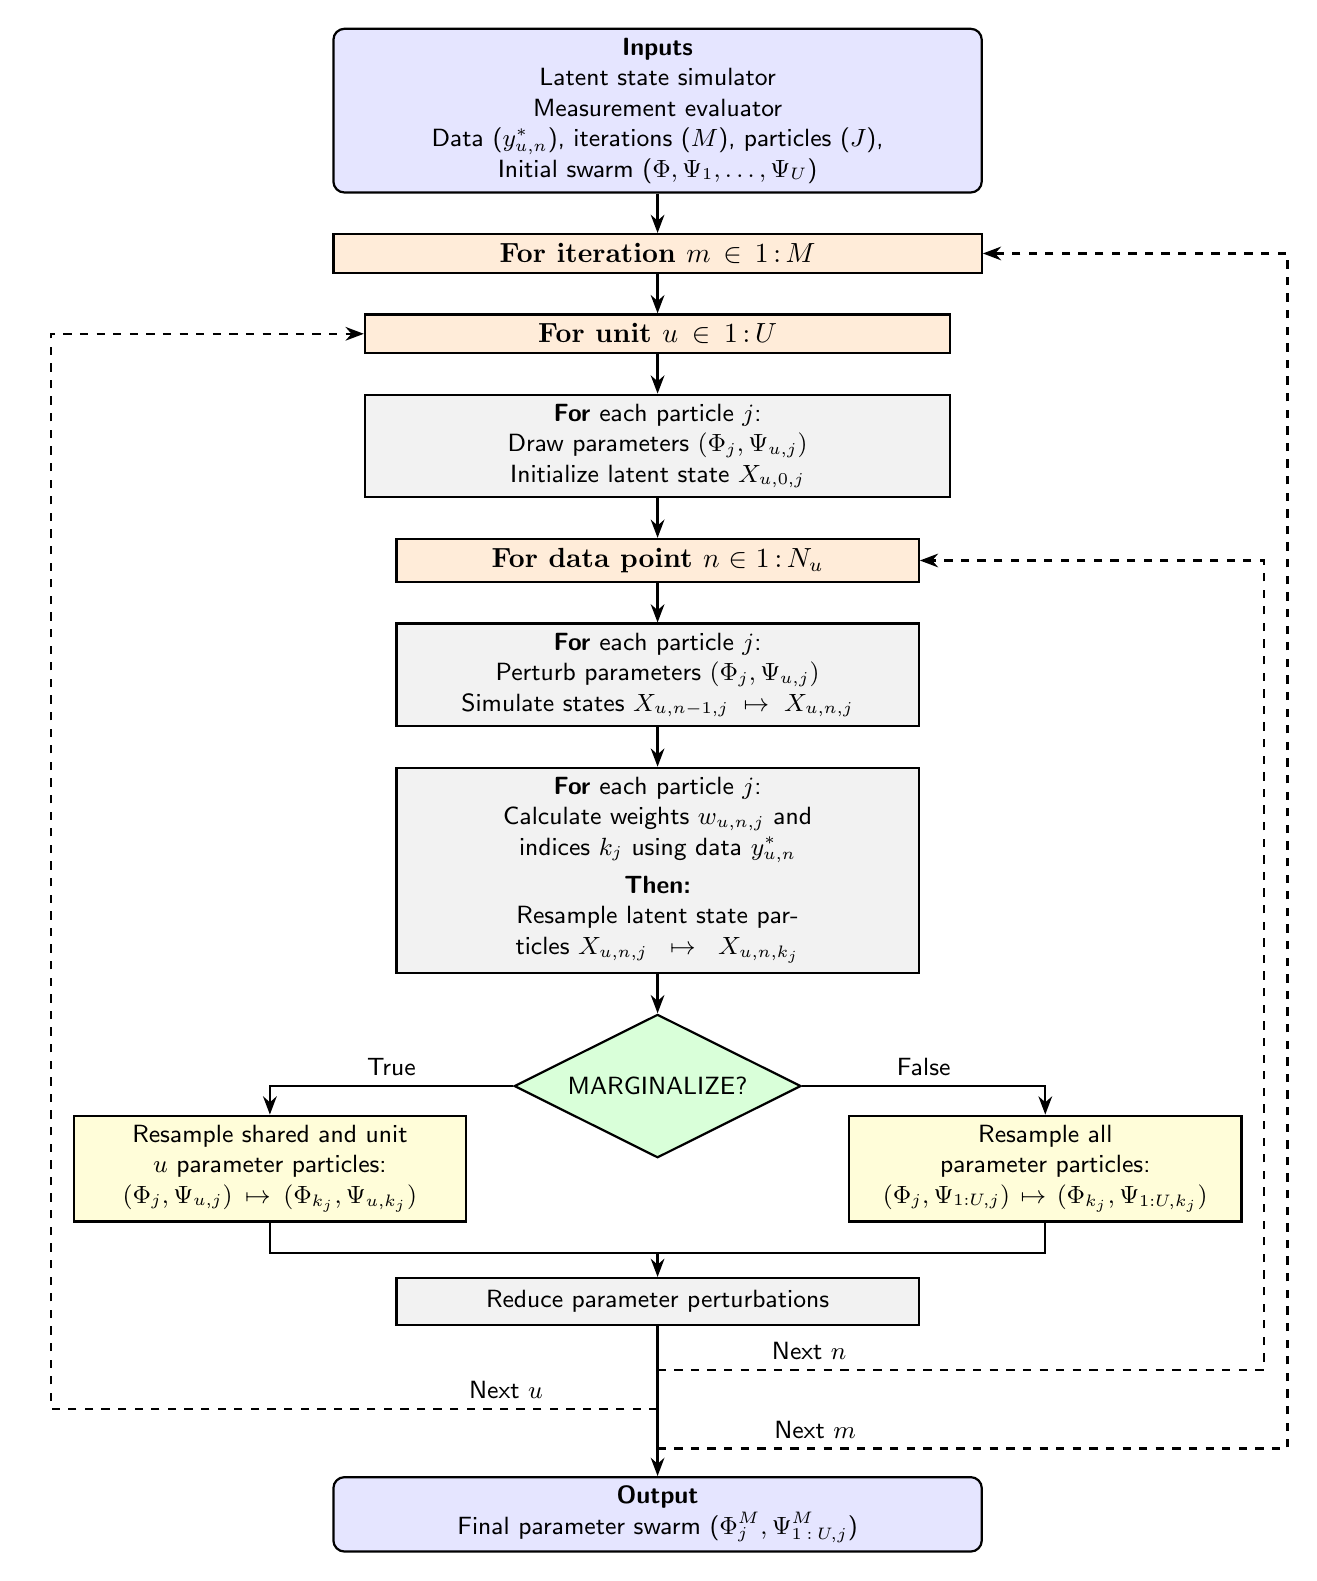
\begin{tikzpicture}[
    font=\sffamily\small,
    >=Stealth,
    node distance=0.5cm and 0.7cm,
    % Base styles for shapes and colors
    io/.style={rectangle, rounded corners, draw=black, thick, fill=blue!10, align=center, minimum height=0.8cm},
    loopstart/.style={rectangle, draw=black, thick, fill=orange!15, align=center, font=\bfseries},
    process/.style={rectangle, draw=black, thick, fill=gray!10, align=center, minimum height=0.8cm},
    decision/.style={diamond, aspect=2, draw=black, thick, fill=green!15, text width=2.5cm, align=center},
    % Increased text width to 4.5cm for the branches
    branch/.style={rectangle, draw=black, thick, fill=yellow!15, text width=4.75cm, align=center, minimum height=1cm},
    % Size structure styles to indicate nesting
    levelM/.style={text width=8.0cm},
    levelU/.style={text width=7.2cm},
    levelN/.style={text width=6.4cm}
]

% --- Nodes ---
\node [io, levelM] (inputs) {\textbf{Inputs}\\Latent state simulator\\ Measurement evaluator\\ Data ($y_{u,n}^*$), iterations ($\Nmif$), particles ($\Np$),\\Initial swarm ($\Shared, \Specific_1, \ldots, \Specific_U$)};

\node [loopstart, levelM, below=of inputs] (loopM) {For iteration $\nmif \!\!\!\in\!\!\! 1 \mycolon \Nmif$};

\node [loopstart, levelU, below=of loopM] (loopU) {For unit $\unit \!\!\!\in\!\!\! 1 \mycolon \Unit$};

\node [process, levelU, below=of loopU] (init) {\textbf{For} each particle $j$:\\Draw parameters $(\Shared_j, \Specific_{u,j})$\\Initialize latent state $X_{\unit,0,j}$};

\node [loopstart, levelN, below=of init] (loopN) {For data point $\time \!\!\in\!\! 1 \mycolon \Time_{\unit}$};

\node [process, levelN, below=of loopN] (simulate) {\textbf{For} each particle $j$:\\Perturb parameters $(\Phi_j, \Psi_{u,j})$\\Simulate states $X_{\unit,\time-1,j} \mapsto X_{u, n,j}$};

\node [process, levelN, below=of simulate] (update) {\textbf{For} each particle $j$:\\Calculate weights $w_{u, n, j}$ and indices $k_j$ using data $y_{u, n}^*$\\ \vspace{1mm} \textbf{Then:}\\ Resample latent state particles $X_{u, n, j} \mapsto X_{u, n, k_j}$};

\node [decision, below=of update] (marginalize) {MARGINALIZE?};

% Branching nodes (Width increased, xshift pushed out to +/-0.8cm to prevent overlap)
\node [branch, below left=of marginalize, xshift=-0.8cm,yshift=0.6cm] (margTrue) {Resample shared and unit $\unit$ parameter particles:\\ $(\Shared_{j}, \Specific_{\unit, j}) \mapsto (\Shared_{k_j}, \Specific_{\unit, k_j})$};
\node [branch, below right=of marginalize, xshift=0.8cm,yshift=0.6cm] (margFalse) {Resample all \\parameter particles:\\
$(\Shared_{j}, \Specific_{1:U, j}) \mapsto (\Shared_{k_j}, \Specific_{1:U, k_j})$};

% Coordinates and new node to manage loop-backs without extra block height
\coordinate [below=1.2cm of marginalize] (mergeN);
\node [process, levelN, below=0.3cm of mergeN, minimum height=0.6cm] (reduce) {Reduce parameter perturbations};
\coordinate [below=0.55cm of reduce] (retN);
\coordinate [below=0.5cm of retN] (retU);
\coordinate [below=0.5cm of retU] (retM);

\node [io, levelM, below=0.35cm of retM] (output) {\textbf{Output}\\Final parameter swarm ($\Shared_j^\Nmif, \Specific_{1\mycolon\Unit, j}^\Nmif$)};

% --- Arrows ---
\draw [->, thick] (inputs) -- (loopM);
\draw [->, thick] (loopM) -- (loopU);
\draw [->, thick] (loopU) -- (init);
\draw [->, thick] (init) -- (loopN);
\draw [->, thick] (loopN) -- (simulate);
\draw [->, thick] (simulate) -- (update);
\draw [->, thick] (update) -- (marginalize);

% Decision arrows
\draw [->, thick] (marginalize) -| node[above, pos=0.25] {True} (margTrue);
\draw [->, thick] (marginalize) -| node[above, pos=0.25] {False} (margFalse);

% Merge arrows
\draw [thick] (margTrue) |- (mergeN);
\draw [thick] (margFalse) |- (mergeN);

% Center flow to output
\draw [->, thick] (mergeN) -- (reduce);
\draw [thick] (reduce) -- (retN);
\draw [thick] (retN) -- (retU);
\draw [thick] (retU) -- (retM);
\draw [->, thick] (retM) -- (output);

% --- Loop Back-Arrows ---
% n-loop 
\draw [->, thick, dashed] (retN) -- ++(7.7,0) node[above, near start] {Next $\time$} |- (loopN.east);

% u-loop 
\draw [->, thick, dashed] (retU) -- ++(-7.7,0) node[above, near start] {Next $\unit$} |- (loopU.west);

% m-loop 
\draw [->, thick, dashed] (retM) -- ++(8.0,0) node[above, near start] {Next $\nmif$} |- (loopM.east);

\path (-8.0, 0);

\end{tikzpicture}%
}
\caption{Flowchart of the Marginalized panel iterated filter (MPIF) algorithm.}
\label{fig:mpif_flowchart}
\end{figure}

\section{Proof and discussion of Theorem~\ref{theorem:pif}}\label{sec:panelTheory}

  Theorem~\ref{theorem:pif} is a straightforward extension of Theorem~4 of \citet{chen25} to PanelPOMP models.
  Our approach is to express an arbitrary PanelPOMP model as a POMP model using a long format, where the latent and observed processes are stacked one unit after another to describe a single long time series that arises by stacking unit time series data one after another.
  Then, Algorithm~\ref{alg:mpif} is equivalent to applying the theory developed in the appendix of \citet{chen25} to this long POMP model.
  For instance, if the perturbation schedule in Algorithm~\ref{alg:mpif} is chosen to to follow the dynamic approach introduced by the authors, then Theorem~1 is just an application of Theorem~4 of \citet{chen25} to a panel version of the model.

  The stacking argument to prove Theorem~\ref{theorem:pif} follows the approach of \citet{breto20}, who previously introduced the PIF algorithm and extended an existing theory for low-dimensional POMP models \citep{ionides15} to derive theoretical properties of PIF.
  However, the recent work of \citet{chen25} provides convergence results for iterated filtering algorithms under weaker assumptions than \citet{ionides15}.
  Most notably, \citet{chen25} prove convergence of iterated filtering algorithms as the random walk standard deviation for parameter perturbations decreases over time rather than being fixed at a small constant.
  Thus, this approach allows us to provide stronger theoretical results for panel iterated filtering than obtained by \citet{breto20}.

  \begin{proof}
  Recall the basic definition of the joint density of a PanelPOMP model:
  \begin{align}
&f_{X_{0:N}, Y_{1:N}}(x_{0:N}, y_{1:N}; \, \theta) =
\nonumber
\\
& \hspace{20mm} \prod_{u = 1}^Uf_{X_{u, 0}}(x_{u, 0};\, \theta)
\prod_{n = 1}^{N_u}f_{Y_{u, n}|X_{u, n}}(y_{u, n} | x_{u, n} ;\, \theta)f_{X_{u, n} | X_{u, n-1}}(x_{u, n}|x_{u, n-1}; \, \theta). \label{eq:ppompSI}
\end{align}
  We would like to pivot the unit specific processes into a single long process, avoiding the need to loop over the unit $u$.
  We define $S_{\tilde{u}} = \sum_{k = 1}^{\tilde{u}}(N_k + 1)$ to be the sum total number of time-steps (observations + initialization) for units $1$ up to unit $\tilde{u}$, defining $S_0 = 0$.
  We use the sequence $\nstack \in \mathbb{N}$ to map time points and states indexed with $(u, n) \in \seq{1}{U}\times\seq{0}{N_u}$ to a new model with only a single index $\nstack \in \seq{1}{S_U}$, defined by the equation $\nstack = S_{\unit-1} + n + 1$

  Now let $T_{\tilde{u}} = \sum_{k = 1}^{\tilde{u}} (t_{k, N_k} - t_{k, 0})$ for $\tilde{u} \in \seq{1}{U}$, with $T_0 = 0$.
  We now define new latent processes $\tilde{X}$ and $\tilde{Y}$. As the original model allows for continuous time latent process, we write
  First,
  \begin{align}
    \tilde{X}(t) &= X_u(t_{u, 0} + (t - T_u)), \, \text{for} \,\, T_{u-1} \leq t \leq T_u.
  \end{align}
  Letting $\tau_{\nstack} = t_{u, n}$, the latent and observable processes are equivalent to
  \begin{align*}
    \tilde{X}_{\nstack} = \tilde{X}(\tau_{\nstack}) = X_{u, n}, \quad \text{and} \quad \tilde{Y}_{\nstack} = Y_{u, n}.
  \end{align*}
  With this new definition of $\tilde{X}$ and $\tilde{Y}$, we have a new POMP model which has joint density
  \begin{align}
&f_{\tilde{X}_{1:S_U}, \tilde{Y}_{1:S_U}}(x_{1:S_U}, y_{1:S_U}; \, \theta) =  \nonumber
\\
& \hspace{20mm}
f_{\tilde{X}_0}(x_0;\, \theta)\prod_{\nstack = 1}^{S_{U}}f_{\tilde{Y}_{\nstack}|\tilde{X}_\nstack}(y_{\nstack} | x_{\nstack}; \, \theta)f_{\tilde{X}_{\nstack}|\tilde{X}_{\nstack - 1}}(x_{\nstack} | x_{\nstack - 1}; \, \theta), \label{eq:lowPOMP}
  \end{align}
  Using the convention that $n' \mapsto (u,0)$ for any $u$, then $f_{\tilde{Y}_{\nstack}|\tilde{X}_\nstack}(y_{\nstack} | x_{\nstack}; \, \theta) = 1$ and \linebreak $f_{\tilde{X}_{\nstack}|\tilde{X}_{\nstack - 1}}(x_{\nstack} | x_{\nstack - 1}; \, \theta) = f_{X_{u, 0}}(x_{u, 0}; \, \theta)$.

  As defined, Eqs.~\ref{eq:lowPOMP} and \ref{eq:ppompSI} describe the same model, but \ref{eq:lowPOMP} has been written to match the SSM of \citet{chen25}, after adjusting for the choice of initializing at $\tilde{X}_1$ rather than $\tilde{X}_0$.
  We refer to Eq~\ref{eq:lowPOMP} as the \emph{long} format, which is indicative that the model has been expressed as a low-dimensional POMP model with observation times ranging from $1$ to $S_U$, rather than a collection (or product) of POMP models, each with observation times $N_u+1$ for $u \in \seq{1}{U}$.

  This representation allows us to naturally extend the theoretical framework of \citet{chen25} to PanelPOMP models.
  Specifically, Assumption~\ref{assumption:regular} impl\old{y}\new{ies} that the set $\Theta$ is a regular compact set \citep[See Definition~1 of][]{chen25}; Assumptions~\ref{assumption:mle2}--\ref{assumption:mle3} ensure that the density in Eq.~\ref{eq:lowPOMP} corresponds to a state-space model that satisfies the MLE conditions of \citet{chen25}, and Assumption~\ref{assumption:mle1} is used as a uniformity condition across particle representations\new{, satisfying the compact set condition of \citet{chen25} by taking the finite union of the unit-specific compact sets $E_u$.}
  Finally, Assumptions~\ref{assumption:kernel1}--\ref{assumption:kernel4} are applied to the cloned version of Model~\ref{eq:lowPOMP}.
  The process is cloned such that we have a new SSM $\dbtilde{Y}_{\nclone} = Y_{u, n}$, $\dbtilde{X}_{\nclone} = X_{u, n}$, using the mapping $\nclone = (\nmif-1)S_\Unit + S_{\unit-1}+n+1$.
  Assumptions~\ref{assumption:kernel1}--\ref{assumption:kernel4} therefore imply assumptions C1-C3 and C4' of \citet{chen25} for the perturbation kernels of the self organized SSM defined via $\big(\dbtilde{Y}_{\nclone}, \dbtilde{X}_{\nclone}\big)$.
  An alternative version of Assumption~\ref{assumption:kernel4} is also stated in Appendix~A.5 of \citet{chen25}, but here we only present one version for brevity.
  Together, the conditions stated in Appendix~\ref{sec:assumptions} allow for a direct application of of the theory developed by \citet[][Appendix~A]{chen25}, with precise details of applying this theorem to the cloned model given in \citet[Supplement~S7,][]{chen25}.
    \end{proof}

  \noindent \old{Formally, Theorem~\ref{theorem:pif} provides guarantees for several variants of iterated filtering algorithms applied to panel models, where each variant is a change to the perturbation kernel that satisfy the conditions \ref{assumption:kernel1}--\ref{assumption:kernel4}.
  For example, Theorem~4 of Chen et al. (2025) is stated for specific perturbation kernels, such as those based on a normal distribution---a choice that has been used by default in most iterated filtering applications (e.g., Ionides et al., 2015; Fox et al., 2022; Subramanian et al., 2021; Wheeler et al., 2024).
  This theory also applies to the variant of iterated filtering proposed by Chen et al. (2025) where perturbations are only applied when needed in a dynamic fashion.}

  \old{Conditions \ref{assumption:kernel1}--\ref{assumption:kernel4} are difficult to verify in practice, and not} \new{Not} all variants of the algorithm that satisfy \old{this condition} \new{Conditions~\ref{assumption:kernel1}--\ref{assumption:kernel4}} are useful for panel models.
    For instance, multivariate normal perturbations applied \new{to all parameters} at each time point \old{is equivalent to applying IF2 to panel models; this approach generally}\new{would result in severe loss of information for unit-specific parameters for the non-focul units and} lead\old{s} to worse results than the PIF algorithm applied to the same model \citep{breto20}.
    As pointed out in Section~\ref{sec:discussion}, the effect of the perturbation kernel is twofold.
    First, it helps revive particle representations of the intermediate parameter distributions by adding random noise.
    Second, the random noise results in a loss of information by masking the signal from the observed data.
    These competing interests are not addressed in theorems involving iterated filtering algorithms.
    In this case, heuristics are useful for determining suitable perturbation densities.

    The modification of \citet{chen25} that applies perturbations only when needed is an effective approach to address the tradeoff between these competing interests.
    For high-dimensional panel models, however, this modification still leads to a large number of updates of the particle representation of the parameter vector $\psi_{-u}$ using data from unit $u$, which is the primary reason that algorithms like PIF struggle in higher dimensional settings.
    This observation leads to the proposal of the MPIF algorithm, which avoids resampling parameters \old{if little information via the likelihood function} \new{\firsttypo}.
 Combining the dynamic perturbations strategies of \citet{chen25} with a marginalization step may also result in an improved algorithm in some cases.
 However, we find that the default multivariate normal perturbations with singular covariance matrix to avoid perturbing all parameters at each time step to be sufficient for parameter estimation in practice.

One reason that Theorem~\ref{theorem:pif} cannot be used directly to infer the practicality of iterated filtering algorithms for panel data is because the behavior of $C_M$ as $M \rightarrow \infty$ is unknown.
Previous works on high-dimensional particle filtering---without adding perturbations or performing data cloning---suggest that the sequence $C_M$ scales exponentially with the number of units \citep{snyder08,bengtsson08}.
While this problem has partially been avoided by writing the PanelPOMP in a long format, which reduces the size of both the latent and observed spaces at each time point, the parameter space for $\Theta$ remains large.
Specifically, the total dimension of $\Theta$ is $\nshared + U\nspecific$, where $\nshared$ and $\nspecific$ are the number of shared and unit-specific parameters, respectively.

Because particle filters are known to perform poorly in high-dimensions, alternative filtering algorithms should be used.
One such example is called the block particle filter \citep{rebeschini15}; this algorithm breaks the state-space into separate units called \emph{blocks}, and performs the update step in the filtering equation independently on each block.
Block particle filters have been found to be effective in high-dimensional settings where the units can be treated as approximately independent.
These results also provides an alternative motivation and justification for the MPIF algorithm, and a potential avenue for expanding Theorem~\ref{theorem:GG} to more general state space models.
In the panel model setting, the MPIF algorithm takes a similar approach to the block particle filter by updating the filtering distribution over the independent units, though the blocking occurs in the parameters space $\Theta$ rather than the latent space $\mathcal{X}$.
Thus, the MPIF algorithm has many similarities to other iterated block particle filtering algorithms that have been effective for moderately sized dynamic systems with spatial coupling \citep{ning23,ionides24}.

\section{Proof of Theorem~\ref{theorem:GG}}\label{appendix:Gaus}

As a reminder, we assume that there are $U\geq 2$ units, labeled $\seq{1}{U}$, with the data for unit $u$ being denoted as $\bm{y}^*_u$.
We write $\theta = (\phi, \psi_1, \ldots, \psi_U)$, and recall that the unit likelihood $L_{u}(\theta;\bm{y}^*_u)$ for unit $u \in 1:U$ depends only on the shared parameter $\phi$ and the unit-specific parameter $\psi_u$.
The panel assumption implies that, conditioned on the parameter vector, the units are dynamically independent.
Therefore, we can decompose the likelihood function for the entire collection of data $L(\theta; \bm{y}^*)$ as:
\begin{align*}
    L(\theta; \bm{y}^*) = \prod_{u = 1}^U L_u(\theta;\bm{y}_u^*) = \prod_{u = 1}^U L_u(\phi, \psi_u;\bm{y}_u^*).
\end{align*}

Each iteration of the Eqs.~\ref{eq:margBayes} and \ref{eq:MPIFupdate} corresponds to a Bayes update followed by a marginalization.
Under the statement of Theorem~\ref{theorem:GG}, the prior and likelihood are assumed to be Gaussian.
In this setting, it is well known that the resulting Bayes posterior also corresponds to a Gaussian distribution.
Similarly, the marginalization of a multivariate Gaussian distribution also results in multivariate Gaussian distributions.
Thus, each iteration of Eqs.~\ref{eq:margBayes} and \ref{eq:MPIFupdate} results in a density that corresponds to a Gaussian distribution.

We now show that the mean of the resulting Gaussian distribution converges to the MLE, while the covariance matrix converges to the zero matrix, resulting in a density with all mass centered at the MLE.
To aid this calculation, we introduce the following lemma.
\begin{lemma}\label{lemma:bound}
\label{lemma:matrix}
  Let $d$ be a positive integer, and let $B_k \in \R^{2\times 2}$ for $k \in \seq{1}{d}$ be a collection of real-valued matrices.
  We construct a sequence of matrices $A_{k} \in \R^{d+1\times d+1}$ such that:
  \begin{equation*}
    \spacingset{1.5}
    [A_k]_{i, j} = \begin{cases}
        [B_k]_{1,1}, & i = j = 1 \\
        [B_k]_{1,2}, & i = 1, j = k+1 \\
        [B_k]_{2, 1}, & i = k+1, j=1 \\
        [B_k]_{2,2}, & i = j = k+1 \\
        1, & i = j, \, i \notin \{1, k+1\} \\
        0, & \text{otherwise}
	\end{cases}
  \end{equation*}
 That is, $A_k$ is a perturbation of the identity matrix, where the first and $(k+1)$th row and column have been modified on the diagonal and on their off-diagonal intersection to match the matrix $B_k$.
If for all $k \in \seq{1}{d}$, $\|B_k\|_2 \leq c$ for some constant $0 < \lemmaBound \leq 1$, then
\begin{equation}\label{eq:lemma:bound}
\bigg\| \prod_{k = 1}^d A_k \bigg\|_2 \leq \lemmaBound.
\end{equation}
\end{lemma}
\begin{proof}[Proof of Lemma~\ref{lemma:bound}]
  For $i, j \in \seq{1}{(d+1)}$, denote $\mu_{(i, j)} \in \mathbb{R}^2$ as the sub-vector of $\mu \in \mathbb{R}^{d+1}$ that contains only the $i$ and $j$th elements, and write $\mu_{-(i, j)} \in \mathbb{R}^{d-1}$ to be the sub-vector of $\mu$ after removing these elements.
  By design, the matrix $A_k$ operates only on the sub-vector $\mu_{(1, k+1)}$.
That is, if $B_k \, \mu_{(1, k+1)} = (\tilde{\mu}_{(1)}, \tilde{\mu}_{(k+1)})^T$, then $A_k\mu = (\tilde{\mu}_{(1)}, \mu_{(2)}, \ldots, \tilde{\mu}_{(k + 1)}, \ldots, \mu_{(d+1)})$.
  From this, we see that for positive integer $m \leq d$,
  the first $m$ factors of the product $\prod_{k = 1}^d A_k$ modify only the first $m + 1$ dimensions of a vector $\mu \in \R^{d+1}$.

We proceed by mathematical induction on the dimension size.
Let $\big\{A^{(d)}_k, k\in \seq{1}{d-1}\big\}$ be a collection of matrices satisfying the condition of Lemma~\ref{lemma:bound} for each $d$.
Setting $P_d=\big\|\prod_{k = 1}^{d-1} A^{(d)}_k \big\|_2$, we first observe that Eq.~(\ref{eq:lemma:bound}) holds for $d=2$ as a direct consequence of the condition $\|B_k\|_2 \leq c$.
Suppose inductively that the lemma holds for $d$, so that $P_d\leq\lemmaBound$.
We wish to bound $P_{d+1}$.
We can choose $A^{(d)}_k$ to be the $(d+1)\times (d+1)$ sub-matrix of $A^{(d+1)}_k$ omitting row and column $(d+2)$.
Thus, for $k\in\seq{1}{d}$,
\begin{equation*}
A^{(d+1)}_k =
  \begin{pmatrix}
    A^{(d)}_k & 0 \\
    0 & 1
  \end{pmatrix}.
\end{equation*}
Consider a vector $\mu \in \R^{d+1}$, such that $\|\mu\|_2 \leq 1$.
Let $\tilde{\mu} \in \R^{d}$ be defined by
\begin{equation}
\tilde{\mu} = \bigg[\bigg(\prod_{k = 1}^{d-1} A^{(d+1)}_k\bigg)\mu\bigg]_{(1:d)}
\end{equation}
and notice that we have
\begin{equation}\label{eq:lemma:d}
\tilde{\mu} = \bigg(\prod_{k = 1}^{d-1} A^{(d)}_k\bigg)\mu_{(1:d)}.
\end{equation}
By construction, we have
\begin{align*}
    \bigg|\Big(\prod_{k = 1}^d A^{(d+1)}_k\Big)\mu \bigg|^2_2 &= \bigg|\Big(A^{(d+1)}_d\prod_{k = 1}^{d-1} A^{(d+1)}_k\Big)\mu \bigg|^2_2\\
    &= \big|A^{(d+1)}_d(\tilde{\mu}_{(1:d)}, \mu_{(d+1)})^T\big|^2_2 \\
    &= \big|B^{(d+1)}_d (\tilde{\mu}_1, \mu_{(d+1)})^T\big|^2_2 + \big|\tilde{\mu}_{(1:d)}\big|^2_2 - \tilde{\mu}^2_1.
\end{align*}
Because $\|B^{(d+1)}_d\|_2 \leq \lemmaBound$, $|B^{(d+1)}_d (\tilde{\mu}_1, \mu_{(d+1)})^T|^2_2 \leq \lemmaBound^2|(\tilde{\mu}_1, \mu_{(d+1)})^T|^2_2$.
Furthermore, our inductive hypothesis applied to Eq.~(\ref{eq:lemma:d}) implies that
$|{\tilde{\mu}}_{(1:d)}|^2_2 \leq \lemmaBound^2|\mu_{(1:d)}|^2_2 \leq \lemmaBound^2|\mu|^2_2$.
Therefore,
\begin{align}
    \bigg|\Big(\prod_{k = 1}^d A_k\Big)\mu\bigg|^2_2 &\leq \lemmaBound^2({\tilde{\mu}}^2_1 + \mu_{(d+1)}^2) + \lemmaBound^2(|\mu_{(1:d)}|^2_2) - {\tilde{\mu}}^2_1 \\
    &= (\lemmaBound^2-1){\tilde{\mu}}^2_1 + \lemmaBound^2 |\mu|^2_2
    \\
    \label{eq:lemma:conclusion}
    &\leq \lemmaBound^2 \vert\mu\vert^2_2,
\end{align}
with Eq.~(\ref{eq:lemma:conclusion}) implied by $\lemmaBound \leq 1$, and hence $(\lemmaBound^2-1) \leq 0$.
It follows immediately from Eq.~(\ref{eq:lemma:conclusion}) that $P_{d+1}\le c$, completing the proof.
\end{proof}

We now return to the main argument.

\begin{proof}[Proof of Theorem~\ref{theorem:GG}]
Using the transformation invariance of the MLE, we can suppose without loss of generality that the maximum of the marginal likelihood for unit $u$ is at $\phi, \psi_u = 0$.
To help ease notation, we write the covariance matrix as
$$
\Lambda^*_u = \begin{pmatrix}
    \Lambda^{(u)}_{\phi} & \Lambda_{\phi, u} \\
    \Lambda_{\phi, u} & \Lambda_{u}
\end{pmatrix}.
$$
Let the prior density $\pi_0(\theta)$ correspond to a Gaussian distribution with mean $\mu_0 \in R^{U+1}$ and precision $\Gamma_0 = \Sigma^{-1}_0 \in \R^{U+1\times U+1}$,
\begin{align*}
    \mu_0 = \begin{pmatrix}
        \mu_0^{(\phi)} \\
        \mu_0^{(1)} \\
        \vdots \\
        \mu_0^{(U)}
    \end{pmatrix}, \, \, \hspace{2mm} \Gamma_0 = \begin{pmatrix}
        \tau^{(\phi)}_0 & 0 & \ldots & 0 \\
        0 & \tau^{(1)}_0 & & \vdots \\
        \vdots & & \ddots & 0\\
        0 & \ldots & 0 & \tau^{(U)}_0
    \end{pmatrix}.
\end{align*}

Eqs.~\ref{eq:margBayes} and \ref{eq:MPIFupdate} contain two indices $(\nmif, \unit)$ for the intermediate density function $\pi_{\nmif, \unit}(\theta)$.
The first index ($\nmif \in \mathbb{N}$) counts the number of times data from all units has been used in the Bayes update (Eq.~\ref{eq:margBayes}), and this corresponds to the number of complete iterations of the $\nmif$ loop in Algorithm~\ref{alg:mpif}.
The second index ($\unit \in \seq{1}{U}$) denotes the data from which unit is currently being used to update the density, and we refer to this as a sub-iteration.
In what follows, we assume that $\pi_{\nmif, \unit - 1}(\theta) = \pi_{\nmif - 1, \Unit}(\theta)$ if $\unit = 1$, and use a similar convention for the corresponding mean and covariance that correspond to this intermediate density.

The density after each sub-iteration of Eqs.~\ref{eq:margBayes} and \ref{eq:MPIFupdate} is Gaussian, and the marginalization step ensures that the precision matrix from previous sub-iterations is diagonal.
Using $\mu_{\nmif, \unit-1}$ and $\Gamma_{\nmif, \unit-1}$ to denote the mean and precision after $\nmif$ complete iterations and the $(\unit-1)$th unit-iteration, we write:
\begin{align*}
    \mu_{\nmif, \unit - 1} = \begin{pmatrix}
        \mu_{\nmif, \unit-1}^{(\phi)} \\
        \mu_{\nmif, \unit-1}^{(1)} \\
        \vdots \\
        \mu_{\nmif, \unit-1}^{(\Unit)}
    \end{pmatrix}, \, \, \hspace{2mm} \Gamma_{\nmif, \unit-1} = \begin{pmatrix}
        \tau^{(\phi)}_{\nmif, \unit-1} & 0 & \ldots & 0 \\
        0 & \tau^{(1)}_{\nmif, \unit-1} & & \vdots \\
        \vdots & & \ddots & 0\\
        0 & \ldots & 0 & \tau^{(\Unit)}_{\nmif, \unit-1}
    \end{pmatrix}.
\end{align*}
By design, each sub-iteration $u$ only modifies the elements of the mean and precision that correspond to the shared parameter $\phi$ and the unit specific parameter $\psi_u$. Thus, we use the superscript notation $\mu_{\nmif, \unit}^{(1, k)}$ and $\Gamma_{\nmif, \unit}^{(1, k)}$ to denote the components of the vector $\mu_{\nmif, \unit}$ corresponding to parameters $\phi$ and $\psi_k$, and the $2\times 2$ submatrix of $\Gamma_{\nmif, \unit}$ with the elements corresponding to parameters $\phi$ and $\psi_k$.

Performing the Bayes update to this distribution (Eq.~\ref{eq:margBayes}) results in an unmarginalized precision matrix, which we denote as $\tilde{\Gamma}_{\nmif, \unit}$, where the only modified components are
$$
\tilde{\Gamma}^{(\nmif, \unit)}_{\nmif, \unit} = \Gamma^{(\nmif, \unit)}_{\nmif, \unit-1} + \Lambda_\unit^* = \begin{pmatrix}
  \tau^{(\phi)}_{\nmif, \unit-1} + \Lambda^{(\unit)}_{\phi} & \Lambda_{\phi, \unit} \\
  \Lambda_{\phi, \unit} & \tau^{(\unit)}_{\nmif, \unit-1} + \Lambda_{\unit}
\end{pmatrix}.
$$
The corresponding mean $\tilde{\mu}_{(\nmif, \unit)} = \mu_{(\nmif, \unit)}$, noting that the marginalization procedure (Eq.~\ref{eq:MPIFupdate}) does not affect the mean, remains the same as the previous iteration except for the components
\begin{align}
\begin{split}
    \tilde{\mu}^{(\phi, \unit)}_{\nmif, \unit} &= \big(\tilde{\Gamma}^{(\nmif, \unit)}_{\nmif, \unit}\big)^{-1}\big(\Gamma^{(\nmif, \unit)}_{\nmif, \unit-1} \mu_{\nmif, \unit-1}^{(\phi, u)} + \Lambda_u^* (0, 0)^T\big) \\
   \mu^{(\phi, u)}_{\nmif, \unit} &= \big(\tilde{\Gamma}^{(\phi, u)}_{\nmif, \unit}\big)^{-1}\Gamma^{(\phi, u)}_{\nmif, \unit-1} \mu_{\nmif, \unit-1}^{(\phi, u)} \\
   &= B_{\nmif, \unit} \mu_{\nmif, \unit-1}^{(\phi, u)},
\end{split}\label{eq:submatB}
\end{align}
where $B_{\nmif, \unit} = \big(\tilde{\Gamma}^{(\phi, 1)}_{\nmif, \unit}\big)^{-1}\Gamma^{(\phi, u)}_{\nmif, \unit-1}$ is a $2\times 2$ matrix that provides the update to the first and $(\unit+1)$th components of a vector $\mu \in \mathbb{R}^{\Unit+1}$.
Now by defining matrix $A_{\nmif, \unit}$ to be a perturbation of the $\Unit+1$ identity matrix, such that
\begin{equation*}
\spacingset{1.5}
\big[A_{\nmif, \unit}\big]_{i, j} = \begin{cases}
  [B_{\nmif, \unit}]_{1, 1} & i = j = 1 \\
  [B_{\nmif, \unit}]_{2, 2} & i = j = u+1 \\
  [B_{\nmif, \unit}]_{1, 2} & i = 1, j = k+1 \\
  [B_{\nmif, \unit}]_{2, 1} & i = k+1, j = 1 \\
  1 & i = j, i \notin \{1, k+1\} \\
  0 & \text{otherwise}
\end{cases},
\end{equation*}
We see that for a given precision matrix $\Gamma_{\nmif, \unit-1}$, the a single sub-iteration of Eqs.~\ref{eq:margBayes} and \ref{eq:MPIFupdate} corresponds to a linear update of the mean vector $\mu_{\nmif, \unit-1}$, defined by
\begin{align*}
  \mu_{\nmif, \unit} = A_{\nmif, \unit} \, \mu_{\nmif, \unit-1}.
\end{align*}
Thus, the mean after $M$ complete iterations, denoted by $\mu_{M}$ is calculated by the product of these linear transformations
\begin{align*}
  \mu_M = \bigg(\prod_{\nmif = 1}^M\prod_{u = 1}^U A_{\nmif, \unit}\bigg)\mu_0.
\end{align*}
Thus, the long-term value of $\mu_M$ depends on the long-term behavior of the product of matrices $A_{\nmif, \unit}$.

We now consider the limiting behavior of the precision matrices, which determines the behavior of the matrices $A_{\nmif, \unit}$.
First, we recall that the unmarginalized precision matrix is of the form:
\begin{align*}
  {\tilde{\Gamma}}^{(\nmif, \unit)}_{\nmif, \unit} = \begin{pmatrix}
  \tau^{(\phi)}_{\nmif, \unit-1} + \Lambda^{(u)}_{\phi} & \Lambda_{\phi, u} \\
  \Lambda_{\phi, u} & \tau^{(u)}_{\nmif, \unit-1} + \Lambda_{u}\end{pmatrix}.
\end{align*}
The marginalization step (Eq.~\ref{eq:MPIFupdate}) for Gaussian densities is represented by setting the off-diagonal elements of the covariance matrix to be zero.
Thus, if we generalize this step by writing
\begingroup
\renewcommand{\arraystretch}{0.7}
$
{\tilde{\Gamma}}^{(\nmif, \unit)}_{\nmif, \unit} = \begin{pmatrix}a & b \\ b & d \end{pmatrix},
$
\endgroup then
\begingroup
\renewcommand{\arraystretch}{0.7}
$
\big({\tilde{\Gamma}}^{(\nmif, \unit)}_{\nmif, \unit}\big)^{-1} = \frac{1}{ad - b^2}\begin{pmatrix}d & -b \\ -b & a\end{pmatrix}
$
\endgroup
and the marginalized version of the matrix is
\begingroup
\renewcommand{\arraystretch}{0.7}
$
\big(\Gamma^{(\nmif, \unit)}_{\nmif, \unit}\big)^{-1} =
    \begin{pmatrix} \frac{d}{ad-b^2} & 0 \\ 0 & \frac{a}{ad-b^2}\end{pmatrix};
$
\endgroup
by taking the inverse of this matrix, we get the precision matrix after a unit-update to be
\begingroup
\renewcommand{\arraystretch}{0.7}
$
   \Gamma^{(\nmif, \unit)}_{\nmif, \unit} = \begin{pmatrix} a - \frac{b^2}{d} & 0 \\ 0 & d-\frac{b^2}{a}\end{pmatrix}.
$
\endgroup

Using this general calculation, the precision matrix after the marginalization step is
\begin{align}
 \Gamma^{(\phi, u)}_{\nmif, \unit} &= \begin{pmatrix}
    \tau_{\nmif, \unit-1}^{(\phi)} + \Lambda_{\phi}^{(u)} - \frac{\Lambda_{\phi, u}^2}{\tau_{\nmif, \unit-1}^{(u)} + \Lambda_u} & 0 \\
    0 & \tau_{\nmif, \unit-1}^{(u)} + \Lambda_u - \frac{\Lambda_{\phi, u}^2}{\tau_{\nmif, \unit-1}^{(\phi)} + \Lambda^{(u)}_{\phi}}
   \end{pmatrix} \nonumber \\
   &= \begin{pmatrix}
    \tau_{\nmif, \unit-1}^{(\phi)} + \Lambda_{\phi}^{(u)} - \alpha_{\nmif, \unit} & 0 \\
    0 & \tau_{\nmif, \unit-1}^{(u)} + \Lambda_u - \beta_{\nmif, \unit}
   \end{pmatrix},\label{eq:margPrecision}
\end{align}
with $\alpha_{\nmif, \unit} = \frac{\Lambda_{\phi, u}^2}{\tau_{\nmif, \unit-1}^{(u)} + \Lambda_u}$ and $\beta_{\nmif, \unit} = \frac{\Lambda_{\phi, u}^2}{\tau_{\nmif, \unit-1}^{(\phi)} + \Lambda^{(u)}_{\phi}}$. Because $\Lambda^*_u$ is a positive definite matrix, for all real numbers $c > 0$,
\begin{align*}
    \Lambda_{\phi}^{(u)} > \frac{\Lambda^2_{\phi, u}}{\Lambda_{u}} > \frac{\Lambda^2_{\phi, u}}{c + \Lambda_{u}}
  \end{align*}
And therefore by letting $\alpha = \min_u \big(\Lambda_u - \frac{\Lambda^2_{\phi, u}}{\Lambda^{(u)}_{\phi}}\big) > 0$, we have $\tau_{\nmif, \unit}^{(\phi)} > \tau_{\nmif, \unit-1} + \alpha$ for all $\nmif \in \mathbb{N}$ and $\unit \in \seq{1}{\Unit}$.
By iterating this inequality, we have $\tau_{\nmif, \unit}^{(\phi)} > \tau^{(\phi)}_0 + \nmif\alpha$, and thus we see that $\tau_{\nmif, \unit}^{(\phi)} = O(\nmif)$.
Therefore as $\nmif \rightarrow \infty$, $\tau_{\nmif, \unit}^{(\phi)} \rightarrow \infty$.
A similar calculation shows that $\tau_{\nmif, k}^{(\unit)} = O(\nmif)$ for all $k, \unit \in \seq{1}{\Unit}$.
Thus, the covariance matrix after $\nmif$ complete iterations has zeros on off-diagonal elements, and the diagonal elements are of order $O(1/\nmif)$, proving the statement in Theorem~\ref{theorem:GG} that $\|\Sigma_\nmif\|_2 \rightarrow 0$.
To finish the proof, we need to show that $|\mu_\nmif|_2 \rightarrow 0$.
To do this, we need more precise descriptions for the rates at which the precision grows.

Our previous calculations establish that both $\tau^{(\phi)}_{\nmif, k}$ and $\tau^{(\unit)}_{\nmif, k}$ are strictly increasing sequences in both $\nmif$ and $k$, and are unbounded.
Thus, the correction terms $\alpha_{\nmif, \unit}$ and $\beta_{\nmif, \unit}$ converge to zero, as the only moving parts are the precision terms that are in the denominator of each of these sequences.
Furthermore, the sequence $\{\alpha_i\}$, defined as
\begin{align*}
  \alpha_i = \sum_{u = 1}^U \alpha_{i, u}
\end{align*}
satisfies $\alpha_i \rightarrow 0$.
Thus, by iterating Eq.~\ref{eq:margPrecision}, we can express the precision matrix after $\nmif$ complete iterations as
\begin{align*}
  \Gamma^{(\phi, u)}_{\nmif} = \Gamma^{(\phi, \unit)}_{\nmif-1, \Unit} = \begin{pmatrix}
    \tau^{(\phi)}_{0} + \nmif\sum_{k = 1}^{\Unit}\Lambda^{(k)}_{\phi} - \sum_{i = 1}^\nmif\alpha_{i} & 0 \\
    0 & \tau^{(\unit)}_{0} + \nmif\Lambda_{k} - \sum_{i = 1}^\nmif \beta_{i, \unit}
  \end{pmatrix}.
\end{align*}
Using the fact that the Ces\`aro mean of a convergent sequence converges to the same limit as the sequence, we have $\frac{1}{\nmif}\sum_{i = 1}^\nmif \alpha_{i} \rightarrow 0$, and therefore
\begin{align}
  \Gamma^{(\phi, k)}_{\nmif, \unit} &= \begin{pmatrix}
    \nmif\sum_{k = 1}^\Unit \Lambda_{\phi}^{(k)} + o(\nmif) & 0 \\
    0 & \nmif\Lambda_k + o(\nmif)
  \end{pmatrix}. \label{eq:nGamma}
\end{align}

Using the rates established in Eq.~\ref{eq:nGamma}, we now investigate the long-term behavior of the mean vector $\mu_\nmif$ by considering the spectral norm of the matrices $B_{\nmif, \unit}$ that define the linear updates to the sub-vector $\mu^{(\phi, \unit)}_{\nmif}$.
Recall from Eq.~\ref{eq:submatB} that $B_{\nmif, \unit} = \big(\Gamma^{(\phi, u)}_{\nmif, \unit-1} + \Lambda^*_{u}\big)^{-1}\Gamma^{(\phi, u)}_{\nmif, \unit-1}$.
We can take advantage of the fact that $\Gamma^{(\phi, u)}_{\nmif, \unit-1}$ is a diagonal matrix to write
\begin{align*}
  B_{\nmif, \unit} &= \big(\Gamma^{(\phi, u)}_{\nmif, \unit-1} + \Lambda^*_{u}\big)^{-1}\Gamma^{(\phi, u)}_{\nmif, \unit-1} \\
  &= \Big(I + (\Gamma^{(\phi, u)}_{\nmif, \unit-1})^{-1}\Lambda^*_{u}\Big)^{-1} \\
  &= \begin{pmatrix} 1 + \frac{\Lambda^{(u)}_{\phi}}{\nmif\sum_{k = 1}^U\Lambda^{(k)}_{\phi} + o(\nmif)} & \frac{\Lambda_{\phi, u}}{\nmif\sum_{k = 1}^U\Lambda^{(k)}_{\phi} + o(\nmif)} \\
  \frac{\Lambda_{\phi, u}}{\nmif\Lambda_u + o(\nmif)} & 1 + \frac{\Lambda_{u}}{\nmif\Lambda_u + o(\nmif)} \end{pmatrix}^{-1} \\
  &= \begin{pmatrix} 1 + \frac{\Lambda^{(u)}_{\phi}}{\nmif\sum_{k = 1}^U\Lambda^{(k)}_{\phi}} + o(1/\nmif) & \frac{\Lambda_{\phi, u}}{\nmif\sum_{k = 1}^U\Lambda^{(k)}_{\phi}} + o(1/\nmif)\\
  \frac{\Lambda_{\phi, u}}{\nmif\Lambda_u} + o(1/\nmif) & 1 + \frac{1}{\nmif} + o(1/\nmif) \end{pmatrix}^{-1}.
\end{align*}
Next we would like to calculate the spectral norm of $B_{\nmif, \unit}$.
Recall that for an invertible matrix $A$, $\|A^{-1}\|_2 = \sigma_{\max}(A^{-1}) = 1 / \sigma_{\min}(A)$, where $\sigma_{\max}$ and $\sigma_{\min}$ correspond to the maximum and minimum singular values of $A$.
Therefore in order to calculate $\|B_{\nmif, \unit}\|_2$, we need to find the minimum singular value of $B^{-1}_{\nmif, \unit}$, which is equal to the minimum eigenvalue of the matrix $B^{-T}_{\nmif, \unit}B^{-1}_{\nmif, \unit}$:
\begin{align*}
  B^{-T}_{\nmif, \unit}B^{-1}_{\nmif, \unit} &= \begin{pmatrix} 1 + \frac{2\Lambda^{(u)}_{\phi}}{\nmif\sum_{k = 1}^U\Lambda^{(k)}_{\phi}} + o(1/\nmif) & \frac{\Lambda_{\phi, u}}{\nmif} \big(\frac{1}{\sum_{k = 1}^U\Lambda^{(k)}_{\phi}} + \frac{1}{\Lambda_u}\big) + o(1/\nmif)\\
  \frac{\Lambda_{\phi, u}}{\nmif} \big(\frac{1}{\sum_{k = 1}^U\Lambda^{(k)}_{\phi}} + \frac{1}{\Lambda_u}\big) + o(1/\nmif) & 1 + \frac{2}{\nmif} + o(1/\nmif) \end{pmatrix} \\
  &= I + \frac{1}{\nmif}\begin{pmatrix} \frac{2\Lambda^{(u)}_{\phi}}{\sum_{k = 1}^U\Lambda^{(k)}_{\phi}} + o(1) & \Lambda_{\phi, u} \big(\frac{1}{\sum_{k = 1}^U\Lambda^{(k)}_{\phi}} + \frac{1}{\Lambda_u}\big) + o(1)\\
  \Lambda_{\phi, u} \big(\frac{1}{\sum_{k = 1}^U\Lambda^{(k)}_{\phi}} + \frac{1}{\Lambda_u}\big) + o(1) & 2 + o(1) \end{pmatrix} \\
  &= I + \frac{1}{\nmif}C_{\nmif, \unit}.
\end{align*}
Using this expression, the eigenvalues of $B^{-T}_{\nmif, \unit}B^{-1}_{\nmif, \unit}$ are equal to one plus the eigenvalues of $\frac{1}{\nmif}C_{\nmif, \unit}$.
Thus, we consider the characteristic polynomial defined by $\det (C_{\nmif, \unit} - \lambda I)$ to calculate the eigenvalues of $C_{\nmif, \unit}$. The resulting polynomial is
\begin{align*}
f_{\nmif, \unit}(\lambda) &=
  \bigg(
    \frac{2\Lambda^{(u)}_{\phi}}{\sum_{k = 1}^U\Lambda^{(k)}_{\phi}} - \lambda\bigg)
  \big(2 - \lambda\big) -
  \Lambda_{\phi, u}^2
  \bigg(
    \frac{1}{\sum_{k = 1}^U\Lambda^{(k)}_{\phi}} + \frac{1}{\Lambda_u}
  \bigg)^2 + o(1)
  \\
  &= \lambda^2 -
  2\bigg(
    1 + \frac{\Lambda^{(u)}_{\phi}}{\sum_{k = 1}^U\Lambda^{(k)}_{\phi}}
  \bigg)
  \lambda +
  \bigg\{
    \frac{4\Lambda^{(u)}_{\phi}}{\sum_{k = 1}^U\Lambda^{(k)}_{\phi}}
    - \Lambda_{\phi, u}^2
    \bigg(
      \frac{1}{\sum_{k = 1}^U\Lambda^{(k)}_{\phi}} + \frac{1}{\Lambda_u}
    \bigg)^2
  \bigg\} + o(1).
\end{align*}
We now proceed by showing that, under the condition specified in Assumption~\ref{eq:GausAssumption}, all roots of the polynomial $f_{\nmif, \unit}(\lambda)$ are strictly positive.
That is, for some $0 < \lambda^{(1)}_{\nmif, \unit} < \lambda^{(2)}_{\nmif, \unit}$, we have the eigenvalues of $C_{\nmif, \unit}$ are $\lambda^{(1)}_{\nmif, \unit} + o(1)$ and $\lambda^{(2)}_{\nmif, \unit} + o(1)$.

For this to hold, we need first that the discriminant of the resulting quadratic equation to be strictly positive.
This condition holds without any assumptions, as we can write the condition as
\begin{align*}
\bigg(2\bigg[ 1 + \frac{\Lambda^{(u)}_{\phi}}{\sum_{k = 1}^U\Lambda^{(k)}_{\phi}}\bigg]\bigg)^2 - &4\bigg(\frac{4\Lambda^{(u)}_{\phi}}{\sum_{k = 1}^U\Lambda^{(k)}_{\phi}} - \Lambda_{\phi, u}^2\bigg[\frac{1}{\sum_{k = 1}^U\Lambda^{(k)}_{\phi}} + \frac{1}{\Lambda_u}\bigg]^2\bigg) > 0 \iff \\
\Lambda^{2}_{\phi, u}\bigg(&\frac{1}{\sum_{k = 1}^U \Lambda_{\phi}^{(k)}} + \frac{1}{\Lambda_u}\bigg)^2 > -\frac{\big(\sum_{k = 1}^U \Lambda_{\phi}^{(k)} - \Lambda_\phi^{(u)}\big)^2}{\big(\sum_{k = 1}^U \Lambda_{\phi}^{(k)}\big)}.
\end{align*}
This condition always holds as the left-hand side of the inequality is strictly positive, and the right-hand side of the inequality is strictly negative.
Thus, the polynomial $f_{\nmif, \unit}(\lambda)$ has two unique real roots.

Next, by taking the derivative and setting equal to zero, we note that $\argmin_\lambda f_{\nmif, \unit}(\lambda) = \lambda^* > 0$, as the coefficient on the linear term of the polynomial is always negative.
This combined with the previous condition ensures that $\lambda^{(2)}_{\nmif, \unit} > 0$.

Finally, if $f_{\nmif, \unit}(0) > 0$, then the intermediate value theorem implies that because $f_{\nmif, \unit}(\lambda^*) < 0$, then there exists some $\lambda^{(1)}_{\nmif, \unit} \in (0, \lambda^{*})$ such that $f_{\nmif, \unit}(\lambda^{(1)}_{\nmif, \unit}) = 0$, implying that $\lambda^{(1)}_{\nmif, \unit}$ is a positive root.
Therefore we need
$$
\frac{4\Lambda^{(u)}_{\phi}}{\sum_{k = 1}^U\Lambda^{(k)}_{\phi}} - \Lambda_{\phi, u}^2\bigg(\frac{1}{\sum_{k = 1}^U\Lambda^{(k)}_{\phi}} + \frac{1}{\Lambda_u}\bigg)^2 > 0,
$$
which is equivalent to the condition
\begin{align*}
  \Lambda_{\phi, u}^2 < \frac{4\Lambda^{(u)}_\phi\Lambda^2_{u}\sum_{k = 1}^U \Lambda_{\phi}^{(k)}}{\big(\Lambda_u + \sum_{k = 1}^{U}\Lambda^{(k)}_{\phi}\big)^2}.
\end{align*}
This condition is guaranteed by Assumption~\ref{eq:GausAssumption}, ensuring that the eigenvalues of $C_{\nmif, \unit}$ are $\lambda^{(1)}_{\nmif, \unit} + o(1)$ and $\lambda^{(1)}_{\nmif, \unit} + o(1)$ for two positive numbers $\lambda^{(1)}_{\nmif, \unit}$ and $\lambda^{(1)}_{\nmif, \unit}$.
As a result of this computation, The minimum eigenvalue of $B^{-T}_{\nmif, \unit}B^{-1}_{\nmif, \unit}$ is equal to $1 + \frac{\lambda^{(1)}_{\nmif, \unit}}{\nmif} + o(1/\nmif)$, implying that
\begin{align*}
  \big\| B_{\nmif, \unit}\big\|_2 &= 1 / \sigma_{min}\big(B^{-1} \big) \\
  &= \frac{1}{1 + 1 + \frac{\lambda^{(1)}_{\nmif, \unit}}{\nmif} + o(1/\nmif)} \\
  &= 1 - \frac{\lambda^{(1)}_{\nmif, \unit}}{\nmif} + o(1/\nmif).
\end{align*}
By Lemma~\ref{lemma:matrix}, we have for all $\nmif \in \mathbb{N}$, $\|\prod_{u = 1}^U A_{\nmif, \unit}\|_2 \leq 1 - \frac{\max_u \lambda^{(1)}_{\nmif, \unit}}{\nmif} + o(1/\nmif)$, and therefore by the sub-multiplicative property of the spectral norm,
\begin{align*}
  \Big\| \prod_{i = 1}^m \prod_{u = 1}^U A_{i, u}\Big\|_2 & \leq \prod_{i = 1}^m \Big\|\prod_{u = 1}^U A_{i, u}\Big\|_2 \\
  &< \prod_{i = 1}^m \Big(1 - \frac{\max_u \lambda^{(1)}_{i, \unit}}{i} + o(1/i)\Big) \rightarrow 0.
\end{align*}
Therefore for any arbitrary initial conditions $\mu_0$ and $\Gamma_0$, we have
$$|\mu_m|_2 = \bigg|\bigg(\prod_{i = 1}^m\prod_{u = 1}^U A_{i, \unit}\bigg)\mu_0\bigg|_2 \rightarrow 0$$
as $m\rightarrow \infty$, completing the proof.
\end{proof}

  \subsection{Proof of Corollary~\ref{corollary:perturbed}}\label{appendix:perturbed}

  For this corollary, we use the same setup as Appendix~\ref{appendix:Gaus}.
  At each step, we add independent random perturbations to the current parameter distribution via a convolution operation before updating using Bayes rule.
  Because Gaussian density convolved with another Gaussian density is still Gaussian, we again only record the mean and precision corresponding to the resulting Gaussian distribution at each step, which we denote $\mu'_{\nmif} \in \R^{U+1}$ and $\Gamma'_{\nmif} \in \R^{U+1\times U+1}$.

\begin{proof}
Let $\mu_{\nmif, \unit} \in \R^{U+1}$ and
$\Gamma_{\nmif, \unit} = \text{diag}
  \big(
    \tau_{\nmif, \unit}^{(\phi)}, \tau_{(\nmif, \unit)}^{(1)}, \ldots, \tau_{(\nmif, \unit)}^{(U)}
  \big)
  \in \R^{U+1\times U+1}$
denote the mean and precision matrices of the multivariate Gaussian after the $(\nmif, \unit)$th iteration.
Consider the $(\nmif, \unit)$th update of Eqs.~\ref{eq:margBayesPerturb}--\ref{eq:MPIFupdatePerturb}.
Using well-known results on the convolution of Gaussian densities and the conjugate prior identities, the umarginalized precision is evaluated as
\begin{align*}
\tilde{\Gamma}'_{\nmif, \unit+1} &= \begin{pmatrix} \frac{\tau_{\nmif, \unit}^{(\phi)}\tau_{\nmif, \unit}^{(\sigma)}}{\tau_{\nmif, \unit}^{(\phi)} + \tau_{\nmif, \unit}^{(\sigma)}} + \Lambda^{(u)}_\phi & \Lambda_{\phi, u} \\ \Lambda_{\phi, u} & \frac{\tau_{\nmif, \unit}^{(u)}\tau_{\nmif, \unit}^{(\sigma)}}{\tau_{\nmif, \unit}^{(u)} + \tau_{\nmif, \unit}^{(\sigma)}} + \Lambda_u\end{pmatrix}.
   \end{align*}
   Following the formula from Appendix~\ref{appendix:Gaus} for finding the marginalized precision matrices, the marginalized precision $\Gamma'_{\nmif, \unit}$ can be expressed as
     \begin{align*}
   \Gamma'_{\nmif, \unit+1} &= \begin{pmatrix} \frac{\tau^{(\phi)}_\nmif\tau^{(\sigma)}_\nmif}{\tau^{(\phi)}_\nmif + \tau^{(\sigma)}_\nmif} + \Lambda^{(\unit)}_{\phi} - \frac{\Lambda^2_{\phi, u}(\tau^{(\sigma)}_\nmif + \tau^{(u)}_\nmif)}{\tau^{(\sigma)}_\nmif\tau^{(\unit)}_\nmif + \Lambda_u(\tau^{(\sigma)}_\nmif + \tau^{(u)}_\nmif)} & 0 \\ 0 & \frac{\tau^{(u)}_\nmif\tau^{(\sigma)}_\nmif}{\tau^{(u)}_\nmif + \tau^{(\sigma)}_\nmif} + \Lambda_{u} - \frac{\Lambda^2_{\phi, u}(\tau^{(\sigma)}_\nmif + \tau^{(\phi)}_\nmif)}{\tau^{(\sigma)}_\nmif\tau^{(\phi)}_\nmif + \Lambda^{(u)}_\phi(\tau^{(\sigma)}_\nmif + \tau^{(\phi)}_\nmif)}\end{pmatrix}.
   \end{align*}
  Because $\Lambda^*_u$ is positive definite, the same argument in the unperturbed case (Appendix~\ref{appendix:Gaus}) gives the existence of positive constants $\{\beta_u, \alpha_u\}_{u = 1}^U$ such that
  \begin{align*}
    \tau^{(\phi)}_{\nmif, \unit+1} &> \frac{\tau^{(\phi)}_\nmif\tau^{(\sigma)}_\nmif}{\tau^{(\phi)}_\nmif + \tau^{(\sigma)}_\nmif} + \alpha_u \\
    \tau^{(u)}_{\nmif, \unit+1} &> \frac{\tau^{(u)}_\nmif\tau^{(\sigma)}_\nmif}{\tau^{(u)}_\nmif + \tau^{(\sigma)}_\nmif} + \beta_u.
  \end{align*}
  Furthermore, the sequence defined by iterating the right hand side of these inequalities is unbounded, which is easily demonstrated by assuming it is bounded, and noting that this leads to a contradiction because $1/\tau^{(\sigma)}_\nmif = o(1/\nmif)$, and therefore each update grows by an amount arbitrarily close to the constants $\alpha_u$ and $\beta_u$.

  Immediately, this result implies that $\tau_{\nmif, \unit}^{(\phi)}, \tau_{\nmif, \unit}^{(u)} \rightarrow \infty$ as $\nmif \rightarrow \infty$.
  That is, the covariance matrix convergence to the zero matrix, even in the presence of parameter perturbations.
  In particular, we can write the correction term
  $$
  \epsilon_{\nmif, \unit} = \frac{\Lambda^2_{\phi, u}(\tau^{(\sigma)}_\nmif + \tau^{(u)}_\nmif)}{\tau^{(\sigma)}_\nmif\tau^{(u)}_\nmif + \Lambda_u(\tau^{(\sigma)}_\nmif + \tau^{(u)}_\nmif)} = o(1),
  $$
  and, using the fact that the sequence $\tau^{(\sigma)}_\nmif$ is defined independently of $\tau^{\phi}_{\nmif, \unit}$, we can write
  \begin{align*}
  \frac{\tau^{(\phi)}_{\nmif, \unit}\tau^{(\sigma)}_\nmif}{\tau^{(\phi)}_{\nmif, \unit} + \tau^{(\sigma)}_\nmif} &= \frac{\tau^{(\phi)}_{\nmif, \unit}}{\frac{1}{\tau^{(\sigma)}_{\nmif}}\big(\tau^{(\phi)}_{\nmif, \unit} + \tau^{(\sigma)}_{\nmif}\big)} \\
  &= \tau_{\nmif, \unit}^{(\phi)}\frac{1}{1+o(1/\nmif)} \\
  &= \tau^{(\phi)}_{\nmif, \unit} + o(1/\nmif).
  \end{align*}
  Thus, the updated precision after a full iteration can be approximated as
  $$
  \tau_{\nmif + 1}^{(\phi)} = \tau^{\phi}_{\nmif} + \nmif\sum_{u = 1}^U \Lambda_{\phi}^{(u)} - \sum_{u = 1}^U\epsilon_{\nmif, \unit} + o(1/\nmif),
  $$
  and therefore
  $$
  \tau_{\nmif + 1}^{(\phi)} = o(\nmif) + \nmif\sum_{u = 1}^U \Lambda_{\phi}^{(u)},
  $$
  and the same basic calculation shows that for all $u$,
  $$
  \tau^{(u)}_{\nmif+1} = o(\nmif) + \nmif\Lambda_{u}.
  $$

Similar to the unperturbed case, the update to the mean can be expressed as $\mu_{\nmif+1} = \big(\prod_{u = 1}^UA'_{\nmif, \unit}\big)\mu_\nmif$, where the matrix $A'_{\nmif, \unit}$ is defined in the same way as $A_{\nmif, \unit}$ from Appendix~\ref{appendix:Gaus}, after replacing the covariance matrices with the perturbed versions:
$$
A'_{\nmif, \unit} = \big(\Gamma'_{\nmif, \unit - 1} + \Lambda^*_u\big)^{-1}\Gamma'_{\nmif, \unit - 1}.
$$
We have shown above that $A'_{\nmif, \unit}$ and $A_{\nmif, \unit}$ are asymptotically equivalent.
Therefore the same argument in the proof of Theorem~\ref{theorem:GG} immediately implies
$$
\big| \mu'_{\nmif} \big|_2 =
  \bigg|
    \bigg(
      \prod_{n = 1}^\nmif\prod_{u = 1}^U A'_{n, u}
    \bigg)
    \mu_0
  \bigg|_2 \rightarrow 0.
$$

   \end{proof}

% \section{Failure Modes and Discussion}\label{appendix:failure}

% \new{Existing theory for iterated filtering (IF) algorithms, including our Theorem~\ref{theorem:pif}, relies on extensions of data cloning (DC) \citep{lele07, ionides15, breto20, chen25}.
% In this approach, iterative Bayesian parameter updates converge to a point mass at the MLE.
% However, our proposed marginalization step (line~\ref{mpif:update} of Algorithm~\ref{alg:mpif}) intentionally breaks from this paradigm to achieve significant computational gains. Consequently, MPIF does not satisfy the conditions of Theorem~\ref{theorem:pif} unless the model contains only unit-specific or shared parameters (where PIF and MPIF are equivalent).
% In this sense, applying MPIF to models with both shared and unit specific parameters represents a potential failure mode of Theorem~\ref{theorem:pif}, though we find that we generally find improved performance over the more theoretically supported PIF algorithm (see Figures~\ref{fig:gomp}--\ref{fig:measles1}).}

% \new{In a standard Bayesian framework, shared parameters, unit-specific parameters, and latent states are all treated as joint random vectors.
% This induces unnecessary dependence among particles, as a defining feature of a panel model (Eqs.~\ref{eq:ppomp}--\ref{eq:ppomp2}) is that latent and observable states are independent across units. MPIF resolves this by decoupling the particles. As a result, successive iterations $(m)$ can no longer be interpreted as a sequence where the previous posterior serves as the next prior. While this decoupling nullifies traditional DC theory, it is precisely this departure from a fully Bayesian treatment that drives the algorithm's efficiency.}
% 
% \new{To develop a theoretical framework to study MPIF, we introduce \emph{marginalized data cloning} (MDC) in Section~\ref{sec:bayes}. Similar to MPIF, MDC decouples shared and unit-specific parameters, but in the simpler setting where likelihoods are available exactly. We provide Theorem~\ref{theorem:GG}, demonstrating that MDC still converges to the MLE under certain conditions, including with systematic parameter perturbations (Corollary~\ref{corollary:perturbed}). In the next section, we explore MDC convergence when the conditions of Theorem~\ref{theorem:GG} are violated. These results indicate that MDC---and consequently, MPIF---likely converges under far weaker assumptions, particularly when intermittent parameter perturbations are included.}

\section{Convergence with highly-coupled Gaussian likelihoods} \label{appendix:GGfail}



\new{Theorem~\ref{theorem:GG} and Corollary~\ref{corollary:perturbed} guarantee convergence of the marginalized data cloning (MDC) algorithm if the unit-likelihood functions are bivariate Gaussian, and are weakly coupled.
In particular, if data are transformed so that the center of the likelihood is the origin and has unit-variance for each component, then the covariance matrix
$$
\Sigma_u = \begin{pmatrix}
1 & \rho \\
\rho & 1 \end{pmatrix}
$$
satisfies $|\rho| < 2 / \big(\sqrt{U}(1 + 1/U)\big)$ for all $u$.
We consider a sequence of simulation studies when this assumption is violated.}

\new{In the first, we consider the case that $U = 100$, and that $\rho = 0.9$ for all units $u$ (the theoretical sufficient condition we derived for $\rho$ in this instance is $|\rho| < 0.198$).
Though the MDC algorithm is not exactly a Bayesian calculation, it does require the specification of a prior distribution to be used as a starting point for the algorithm.
We decide to choose a poorly-informed prior to show that even when the initialized value is far from the truth, and the assumptions of Theorem~\ref{theorem:GG} are not satisfied, the MDC algorithm quickly moves from a poor starting point to a region near the MLE, and subsequently appears to converge to the MLE.
We choose the initial prior for each unit to be bivariate normal, with mean $\mu_{u, 0} = (5, 5)$, and variance $\Sigma_{u, 0} = \text{diag}(1.5, 1.5)$.
In this case, the prior is very poorly chosen as it is highly informative and centered near a point that is very far from the region of high-likelihood.}



\new{Figure~\ref{fig:GGlargeRho} demonstrates that within just a few iterations, the MDC algorithm quickly jumps from its poor starting location to a region of relatively high likelihood---a known feature of iterated filtering algorithms \citep{tan24}.
In the second panel of Figure~\ref{fig:GGlargeRho}, the rate of convergence appears to be of the form $\mathcal{O}\big(m^{-c}\big)$ for some decay rate $c > 0$.
Fitting a linear model to the equation $\log(\phi_m) = \log(A) - c \log(m)$ confirms this behavior, yielding an $R^2 > 0.9999$.
In fact, this model suggests that the asymptotic rate of convergence to the MLE is $\mathcal{O}\big(m^{-(1-|\rho|)}\big)$ for this particular simulation design, as the estimated decay coefficient was $c = 0.1000175 \approx 0.1 = 1-|\rho|$.
Thus, it appears that even when conditions of Theorem~\ref{theorem:GG} are violated, the MDC algorithm converges in the bivariate Gaussian case when all unit-specific covariance matrices share the same correlation parameter $\rho$, though we do not have analytic results that confirm this finding.}

\begin{figure}[ht]
\begin{knitrout}
\definecolor{shadecolor}{rgb}{0.969, 0.969, 0.969}\color{fgcolor}

{\centering \includegraphics[width=\maxwidth]{figure/fig-GGlargeRho-1} 

}


\end{knitrout}
\caption[Convergence with highly coupled Gaussian likelihoods]{\label{fig:GGlargeRho}\new{Convergence of MDC with highly correlated Gaussian unit-likelihoods and poor starting conditions. Convergence of the unit-specific parameter is not shown, but follows the same trajectory.}}
\end{figure}

\new{Expanding this simulation result to different choices of $\rho$ and $U$ further validates these results (Figure~\ref{fig:GGlargeRho2}).
In this figure, we also compare the convergence of MDC to DC, and the perturbed marginal data cloning (PMDC) that is the subject of Corollary~\ref{corollary:perturbed}.
As expected, Figure~\ref{fig:GGlargeRho2} shows that the loss of information that results from the additional marginalization step causes a reduction in convergence rates relative to DC.
However, adding perturbations make the PMDC move from the starting value to the MLE much faster than DC. To ensure that the perturbed data cloning algorithm still converges to a point value, the standard deviation of the perturbations are decreased with rate $o(1/m)$.}


\begin{figure}[ht]
\begin{knitrout}
\definecolor{shadecolor}{rgb}{0.969, 0.969, 0.969}\color{fgcolor}\begin{kframe}


{\ttfamily\noindent\bfseries\color{errorcolor}{\#\# Error in `gzfile()`:\\\#\# ! cannot open the connection}}

{\ttfamily\noindent\bfseries\color{errorcolor}{\#\# Error:\\\#\# ! object 'GaussianFailure' not found}}\end{kframe}
\end{knitrout}
\caption[Convergence with combinations of $U$ and $\rho$]{\label{fig:GGlargeRho2}\new{Convergence of the shared parameter value, $\phi$, towards the true MLE at $\phi = 0$. Shown on a log-scale to emphasize differences in tail convergence rates.}}
\end{figure}

\new{Section~\ref{appendix:Gaus} reveals a fundamental tradeoff in iterative Bayesian procedures: converging to the MLE requires unbounded growth in the precision of the prior at each iteration, yet this growth inherently shrinks the step size towards the MLE.
If precision accumulates too rapidly, the algorithm stalls prematurely.
This explains why PMDC outperforms DC in Figure~\ref{fig:GGlargeRho2}, despite lacking its theoretical guarantees:
injecting noise into the intermediate priors curbs runaway precision, enabling larger, sustained steps toward the MLE.
% This dynamic also illustrates why iterated filtering algorithms are often more computationally efficient than particle Markov chain Monte Carlo (PMCMC) algorithms.
% IF rapidly navigates to high-likelihood spaces by providing large parameter updates at each time step; this avoids the PMCMC bottleneck of requiring a complete data pass evaluated at poor parameter values. These areas of parameter space are statistically irrelevant and algorithmically problematic since they can have high Monte Carlo variance and correspondingly poor MCMC mixing.
% This efficiency is further magnified in panel models, which require high-dimensional joint parameter distributions for a fully Bayesian analysis.
}

\new{Systematic, large correlation between shared and unit specific parameters is not the only scenario where the requirements of Theorem~\ref{theorem:GG} are not met.
A potentially more severe deviation from our derived sufficient conditions is the case where a single unit $u$ has high correlation between $\phi$ and $\psi_u$, whereas the remaining units do not.
Furthermore, we could have a case where the correlation $\rho < 0$.
We expand this fist simulation study to consider both of these scenarios.
First, we set $\rho_{-u} = \pm 1 / \big(\sqrt{U}(1 + 1/U)\big)$ (midway between zero and the derived upper bound for $|\rho|$) randomly selected positive or negative correlation for all units but $u = (U+1)/2$.
For unit $u$, we set $\rho_u$ to be the negative value of the midway point between the upper bound of Theorem~\ref{theorem:GG} and $1$.
We find similar results as our previous simulation study, namely that all three versions of the data cloning algorithm appear to be converging to the MLE.
When some of the correlations are negative, the MDC can outperform the DC algorithm, as was seen in Figure~\ref{fig:DC} of the main text.
In all cases, the perturbed version of the algorithm converges the fastest.
Notably, if the correlations can be both positive and negative for each unit, we have no guarantees that each subsequent step results in a step towards the MLE.}

\begin{figure}[ht]
\begin{knitrout}
\definecolor{shadecolor}{rgb}{0.969, 0.969, 0.969}\color{fgcolor}\begin{kframe}


{\ttfamily\noindent\bfseries\color{errorcolor}{\#\# Error:\\\#\# ! object 'GaussianFailure' not found}}

{\ttfamily\noindent\bfseries\color{errorcolor}{\#\# Error:\\\#\# ! object 'GaussianFailure' not found}}

{\ttfamily\noindent\bfseries\color{errorcolor}{\#\# Error:\\\#\# ! object 'GG2\_2' not found}}

{\ttfamily\noindent\bfseries\color{errorcolor}{\#\# Error:\\\#\# ! object 'GG2\_2' not found}}

{\ttfamily\noindent\bfseries\color{errorcolor}{\#\# Error:\\\#\# ! object 'GG2\_1' not found}}

{\ttfamily\noindent\bfseries\color{errorcolor}{\#\# Error:\\\#\# ! object 'tmp\_fig' not found}}\end{kframe}
\end{knitrout}
\caption[Gaussian convergence with alternating covariance structure]{\label{fig:GGlargeRho3} \new{Shared and unit-specific parameter values for each of the iterated Bayesian updates. Absolute value is taken to ensure positivity, and the logarithm used to enable comparison of convergence rates. Large shifts on the log-scale represent iterations where the estimate for the parameter value switches sign.}}
\end{figure}

\new{Theorem~\ref{theorem:GG} and Corollary~\ref{corollary:perturbed} provide theoretical guarantees when $|\rho_u|$ is bounded. Because MPIF is most advantageous for large panel models, one might worry that this bound depends on the number of units, $U$. Although our simulations suggest this limit may not be strictly necessary, its theoretical implications are worth examining.}

\new{Consider the case where all unit-specific likelihoods share the covariance matrix:
$$\Sigma_u = \begin{pmatrix} 1 & \rho \\ \rho & 1 \end{pmatrix}.$$
By summing the unit-specific precision matrices and inverting the result via the Schur complement, the joint covariance structure of the full panel model becomes: $[\Sigma]_{1, 1} = 1/U$, $[\Sigma]_{i, i} = 1 - \rho^2 + \rho^2 / U$, $[\Sigma]_{1, i} = [\Sigma]_{i, 1} = \rho/U$, and $[\Sigma]_{i, j} = [\Sigma]_{j, i} = \rho^2/U$ for all $i, j \in \{2, 3, \ldots, U+1\}$.
Thus, as $U \to \infty$, the Fisher information for the shared parameter $\phi$ diverges, leading to a degenerate joint likelihood.}

\new{Consequently, the correlation $\rho$ must naturally shrink as $U$ grows to prevent the joint likelihood from harboring infinite precision for the shared parameter.
If infinite precision were present, the convergence behavior of MDC or MPIF would become trivial, as a single iteration would instantly collapse to the MLE of the shared parameter, and remaining iterations are equivalent to the standard DC algorithm.
In short, the bound's dependence on $U$ is not a restrictive algorithmic flaw, but a natural scaling requirement for a properly specified panel likelihood.}


\new{We finally consider the convergence of the MPIF algorithm for nonlinear, non-Gaussian models that have high correlation between shared and unit specific parameters.
One such examples is the stochastic Gompertz models presented in the manuscript.
Here, we focus on the $U = 50$ model of Figure~\ref{fig:gomp}.
Using the extended search results from the creation of confidence intervals in Section~\ref{appendix:ci}, we can plot the output of many Monte Carlo searches for the maximum likelihood.
For this model, each search from unique starting positions quickly converges to a region of high-likelihood.
By plotting output parameters values for these searches, we see that the likelihood surface has ridges in specific dimensions.
For instance, Figure~\ref{fig:ridge} shows that there is a strong relationship between estimated shared parameter $r$ and unit-specific parameters $\tau_u$, suggesting a ridge in the likelihood surface in this two-dimensional direction.
The exact shape of the high-dimensional likelihood surface is not readily available, so we rely on the correlation of estimated values as a proxy.
}

\begin{figure}[ht]
\begin{knitrout}
\definecolor{shadecolor}{rgb}{0.969, 0.969, 0.969}\color{fgcolor}

{\centering \includegraphics[width=\maxwidth]{figure/correlationFig-1} 

}


\end{knitrout}
\caption[Correlation Gompertz model near MLE]{\label{fig:ridge}\new{Estimated values of $r$ and $\tau_1$, based on the profile likelihood evaluation of Figure~\ref{fig:mcap}. The estimated correlation between these parameter estimates is -0.836, which violates the correlation condition of Theorem~\ref{theorem:GG}, yet the MPIF algorithm still reliably obtains the MLE for this model.}}
\end{figure}

% \subsection{Diagnostics and confidence intervals}\label{sec:practical}
% 
% \new{While the preceding sections demonstrate that the MPIF algorithm (Algorithm~\ref{alg:mpif}, Eqs.~\ref{eq:margBayes}--\ref{eq:MPIFupdate}) reliably converges to high-likelihood regions even when the assumptions of Theorems~\ref{theorem:pif} and \ref{theorem:GG} are violated, its primary advantages are practical rather than theoretical. Below, we discuss the practical failure modes and limitations of MPIF, along with strategies to mitigate them.}
% 
% \new{First, while Theorem~\ref{theorem:pif} guarantees asymptotic convergence to the MLE, its conditions are rarely verifiable in practice.
% Though the assumptions can be described as rather weak smoothness conditions of the likelihood function \citep{chen25}, they generally require the ability to evaluate the transition density (see assumptions \ref{assumption:mle1} and \ref{assumption:mle3}).
% Because MPIF is designed specifically for models lacking closed-form transition densities, these theoretical guarantees cannot usually be directly confirmed. 
% For verified single-unit examples, which can readily be extended to multi-unit settings via Section~\ref{sec:panelTheory}, see Supplement~S3 of \citet{chen25}.}
% 
% \new{Second, theoretical convergence is asymptotic in both iterations ($M$) and particles ($J$).
% In practice, finite implementations of PIF typically require computational effort of the order $M=100$ and $J=1000$ to approach the MLE reliably \citep{wale19,ranjeva19,breto20,lee20,domeyer22,panelpomp,yang25}, though the exact effort required varies by model and data.
% Because the algorithm is stochastic by nature, convergence is generally assessed empirically by confirming that additional iterations yield negligible likelihood improvements and that multiple initializations converge to the same likelihood values.
% This process is often aided by parallel computation and Monte Carlo adjusted profile confidence intervals \citep{ionides17}.
% In practice, we recommend starting with a small number of iterations and particles to assess the amount of effort that may be required.
% Notably, the computational effort scales linearly in both $M$ and $J$, making it simple to approximate the time for a larger scale search will take after making a small-scale optimization effort.}




% \new{Finally, a known feature of IF algorithms is that they move to a region of high-likelihood very quickly but are slow to converge to the MLE once in the region of high-likelihood \citep{tan24}.
% This occurs because the same parameter perturbations that prevent particle depletion also introduce information loss as the filter progresses, essentially stalling fast convergence once near the peak.
% This failure mode is exacerbated by long time series---or, in panel models, a large number of units ($U$) acting as a long composite series. Figure~\ref{fig:gomp} illustrates this: for $U = 5$ and $U = 15$, MPIF successfully maximizes the likelihood with just $M = 50$ and $J = 1000$.
% However, for $U = 50$ and $U = 100$, the algorithm falls short of the true maximum by $round(ll_50_diff, 2)$ and $round(ll_100_diff, 2)$ log-likelihood units, respectively (roughly $round(ll_50_diff / 50, 2)$ and $round(ll_100_diff / 100, 2)$ per unit). While the likelihood continues to climbs steadily after 50 iterations, closing this gap requires increasing $M$ to values larger than required for $U \leq 15$.}
% 
% \new{Note that for $U \geq 200$, the parameter space is too large to compute the true maximum via Kalman filter for comparison in the lower half of Figure~\ref{fig:gomp}, though we see that the likelihood of the estimated parameters rapidly climb higher than the likelihood value of the generating parameters, as expected by Wilks' theorem; as the likelihood appears to continue climbing in these large $U$ scenarios, a user in practice would be encourage to continue the search for the MLE by increasing the number of iterations.
% Both the MPIF algorithm and software enable continuation of previous searches, so a user in this case would only need to restart the search from the end of the previous iterations, a common occurrence in practice.
% In addition to increasing computational effort, solutions to the slower convergence rate near the MLE may involve reducing the number of perturbations \citep{chen25}, block-style optimization \citep{breto20,panelpomp}, or the use of recent advances in automatically differentiable particle filters \cite{tan24}.
% Each of these potential modifications can be applied to general IF algorithms, but are greatly enhanced in the panel setting by using the marginalization step introduced in this article.}


\section{Practical inference and confidence intervals}\label{appendix:ci}

\new{The MPIF algorithm provides new simulation based inference capabilities for nonlinear PanelPOMP models, but these capabilities should be complemented by good data analysis practices.
Although Theorems~\ref{theorem:pif} and \ref{theorem:GG} provide asymptotic convergence guarantees for panel iterated filtering algorithms, they are not directly informative in the practical setting when the conditions are not verifiable and a finite number of particles and iterations are used.
Here we provide a few suggestions for practical inference.
Existing tutorials and recommendations for the PIF and IF2 algorithms are abundant \citep{ionides15,king16,breto20,wheeler24,panelpomp,king25,yang25}, and we find similar diagnostic tools and recommendations useful for the newly proposed MPIF algorithm.}

\new{As the goal of the algorithm is maximum likelihood estimation, a key diagnostic tool for convergence is plotting the log-likelihood after each iteration, as was done in Figures~\ref{fig:gomp} and \ref{fig:measles1} of the manuscript.
If the algorithm is working, a user would expect to see log-likelihood values generally increase with each iteration, and slowly converge to a single value.
Bearing in mind the stochastic nature of the algorithm, some variation is to be expected and multiple replications should be carried out.
In addition to monitoring the log-likelihood, it is helpful to plot simultaneously the parameter values at the end of each iteration; this visualization is useful in diagnosing the consistency between replicated searches, and can also help determine if the parameter perturbations are too small (parameter values are change too slowly) or large (irregular fluctuations in parameter values in sequential iterations).
Figures of parameter values and likelihoods over iterations are referred to as \emph{trace plots}.
In Figure~\ref{fig:GompTraces}, for instance, we see that distinct Monte Carlo replicates with unique starting values quickly moves to a region of high-likelihood.
}



\begin{figure}[ht]
\begin{knitrout}
\definecolor{shadecolor}{rgb}{0.969, 0.969, 0.969}\color{fgcolor}

{\centering \includegraphics[width=\maxwidth]{figure/traceFigure-1} 

}


\end{knitrout}
\caption[Convergence diagnostic plot: parameter traces]{\label{fig:GompTraces}\new{Trace plots for the $U=50$ Gompertz model. Values over iteration shown are the log-likelihood, shared parameters $r$ and $\sigma$, and a single unit-specific parameter $\tau_{30}$. The log-likelihood panel of this figure appears to be steadily climbing after 50 iterations, suggesting more computational effort may be required to fully maximize the likelihood function.
Because of the large increase in likelihood relative to random initializations within the first few iterations, plotting the likelihood and parameter values after the first few iterations (Panel B) helps visualize smaller changes and diagnose performance in later iterations.}}
\end{figure}

\new{Convergence diagnostics and algorithmic performance is generally enhanced by repeating the optimization procedure for multiple starting locations.
In this case, finite sample properties are supported by many of the distinct Monte Carlo replicates of the algorithm converging to the same likelihood values (Figure~\ref{fig:gomp} and \ref{fig:measles1}).
Even simple POMP models can have multi-model likelihood surfaces \citep{auger16,wheeler25}, in which case there may be two or more regions of high-likelihood in the parameter space to which individual trajectories converge.
Monte Carlo replicates can be computed in an embarrassingly parallel fashion \citep{foster95}, so it is relatively straightforward to take advantage of available computing resources.
Sufficient replicates should be run to evaluate consistency among the highest-performing results: substantial variation in log-likelihoods among the top runs suggests that additional replicates could yield better outcomes, whereas stability indicates that an optimal threshold has likely been reached.
The number of searches could be set to the number of available computing cores, which may be of order 100 in scientific computing environments.}

\new{Iterated filtering algorithms require the specification of various hyperparameters: the number of particles, $J$; the number of iterations, $M$; aand the size of parameter perturbations.
The number of particles $J$ should be sufficiently large as to avoid issues of particle depletion and provide reasonable approximations to the likelihood function.
This can be done by plotting the effective sample size (ESS) \citep{liu01book}, or checking for consistent behavior in trace plots.
Similarly, the number of iterations $M$ should be sufficiently large so that additional iterations are not expected to increase the likelihood further, and trace plots are useful in this regard.
Though each model and dataset may require distinct specifications for $J$ and $M$, we generally find that $J$ on the order of $1000$ particles and $M$ on the order of $100$ iterations is sufficient for many problems and a useful starting point.
However, prior to performing a large computation, it is useful to perform a much smaller computation to assess what level of computation is required for the current task, and how long such a calculation may take.
For a fixed dataset and model, PIF and MPIF scale linearly in both $J$ and $M$, so a smaller initial trial (e.g., $J = 100$ and $M = 5$) can be used to determine how long a larger computation will take; for instance, a single Monte Carlo run with $J = 1000$ and $M = 100$ would require approximately $10\times 20 = 200$ times the computation effort as a $J = 100, M = 5$ search.
If a user finds that the choice of $M$ or $J$ was not sufficient for convergence, existing software packages like the panelPomp R package and the Pypomp Python package enable continuation of the search from the last point rather than starting from initial values.}

\new{Parameter perturbations should be sufficiently large that the parameter values can move from a region of low-likelihood to one of high-likelihood, but small enough that information from previous observations is not routinely lost.
Furthermore, in order to converge to a point, parameter perturbations should shrink over time.
Though the theory permits various choices for the perturbation kernel, mean zero additive Gaussian noise is typically used in practice.
Useful choices for parameters that must remain positive (such as transition rates) and are therefore fit on a log-scale is an initial perturbation size $\sigma = 0.02$, and perturbations are decreased following a geometric cooling rate (See \citet{king16} for more details).
Optimal choices for the initial perturbation size and cooling schedule are model and data specific, and may require experimentation or attention to convergence diagnostic plots.
However, we find that this default choice is adequate in many situations.}

\new{Once a parameter estimate has been obtained, the computation of confidence intervals can further help validate and diagnose parameter estimates.
The primary means of constructing confidence intervals for PanelPOMP models is the Monte Carlo adjusted profile (MCAP) \citep{ionides17}.
Profile likelihoods are an effective tool for obtaining univariate confidence intervals for complex models \citep{pawitan01}, and MCAP adjusts these confidence intervals to account for the Monte Carlo nature of both the parameter estimation and likelihood evaluation.
These intervals are computed for PanelPOMP models by fixing a target parameter at a range of pre-specified values, and performing a maximum likelihood search for the remaining parameter values.
This is demonstrated for the two shared parameters, $\sigma$ and $r$, for the $U = 50$ stochastic Gompterz model considered in the manuscript.
The choice of $U = 50$ was selected as it appears to be the model and data where convergence of the MPIF algorithm appears most suspect.
The MCAP confidence intervals in Figure~\ref{fig:mcap} show, however, that the optimization approach is able to reliably find the MLE and provide confidence intervals.}




\begin{figure}[ht]
\begin{knitrout}
\definecolor{shadecolor}{rgb}{0.969, 0.969, 0.969}\color{fgcolor}

{\centering \includegraphics[width=\maxwidth]{figure/CIfigure-1} 

}


\end{knitrout}
\caption[Monte Carlo adjusted profile confidence intervals]{\label{fig:mcap}\new{MCAP confidence intervals. The horizontal line marks the maximum likelihood obtained by directly optimizing model exact model likelihoods computed using the Kalman Filter; the vertical solid red line marks the MLE; the vertical dashed lines represent the 95\% MCAP confidence interval; and the vertical dotted line is the smoothed estimate based on the MCAP curve.
The parameter values used to generate the data, $r = 0.1$ and $\sigma = 0.1$, both lie in the confidence region.
Fixing the process noise parameter $\sigma$ appears to aid in the optimization, a result that has been observed elsewhere \citep{wheeler24}}}
\end{figure}


\new{For a given amount of computational resources, there is a trade off between the number of searches that can be carried out, the length of each search, and the number of particles, $J$.
For the scientific conclusions of the data analysis, the primary task is to validate that the search procedure is effective, rather than whether it is computationally efficient.
However, improvements in computational efficiency can assist the exploration of variations in the models and data used in the analysis.
Additional strategies can improve computational efficiency, such as multi-stage searches where the most successful preliminary searches are further refined \citep{bhadra11,breto20}.
Any heuristic to assist optimization can be explored and tested, to see if it helps.
Maintaining independence of searches is wise, when a single search is reasonably effective, since it simplifies the interpretation of the resulting parameter estimates.
Since one cannot readily guarantee global optimization of a multimodal non-convex function, a practical guarantee amounts to providing evidence that a focal region of interest has been well searched.
Searches will be initialized in the focal region, but they may leave it and reveal that the focal region was poorly chosen.}

\new{In addition to diagnosing the optimization procedure on the data, it can be useful to validate it on simulated data for which the exact data generating model is known.
Such simulation studies, similar to the one presented here, can readily estimate coverage of confidence intervals and size of tests.
If necessary, the cutoff for a profile confidence interval cutoff or hypothesis test can be adjusted to give the correct behavior on simulated data.
}

\section{Additional measles model details}\label{sec:search_boxes}
\subsection{Parameter Search Boxes}

\new{Initial parameter vectors used in the mechanistic measles models fitted in Section~6 of the main text are sampled uniformly from hyperrectangles. 
Table~\ref{tab:parameter_boxes} summarizes the bounds used to draw the initial parameters for the $c$-shared, $\iota$-shared, and 7-shared (many-shared) models.
We chose these bounds to include a scientifically plausible range of values and to contain the MLEs reported by \citet{he10}. 
For example, because the lowest reported value for $\mathcal{R}_0$ across the 20 cities was 21, and the highest was 57, we set the lower bound to 10 and the upper bound to 60. 
The same bounds are used whether the parameter is shared or unit-specific, and they are the same regardless of the unit. 
$\iota$ is exclusive to the $c$-shared model, and $\iota_1$ and $\iota_2$ are exclusive to the $\iota$-shared and 7-shared models.}

\subsection{Measurement model}

\new{The measurement model is given by a discretized normal distribution for the number of cases reported:
\begin{align*}
 P\big(Y^{(u)}_n = y^{(u)} \big| Z^{(u)}_n = z^{(u)} \big) =
   \Phi\big(y^{(u)} + 0.5, \rho^{(u)} z^{(u)}, \rho^{(u)}(1-\rho^{(u)})z^{(u)} +
     [\psi^{(u)} \, \rho^{(u)} \, z^{(u)}]^2 \big)\\
   \qquad - \Phi\big( y^{(u)} - 0.5, \rho^{(u)} z^{(u)}, \rho^{(u)}(1-\rho^{(u)})z^{(u)} +
     [\psi^{(u)}\, \rho^{(u)}\, z^{(u)}]^2 \big)
\end{align*}
where $\Phi(\cdot;\mu, \sigma^2)$ is the CDF for a $\normal[\mu,\sigma^2]$ random variable and $Z_n$ is the number of people transitioning from compartment $I$ to $R$ between the $(n-1)th$ and $n$th observation times.}

\begin{table}[ht]
\centering
\caption[Bounding box for UK Measles parameter search]{\new{Parameter search boxes showing the lower and upper bounds used for drawing initial parameter values across the three fitted models.}}
\label{tab:parameter_boxes}
\begin{tabular}{lcc}
\hline
Parameter & Lower Bound & Upper Bound \\
\hline
$\mathcal{R}_0$ & 10 & 60 \\
$\rho$ & 0.1 & 0.9 \\
$\sigma_{SE}$ & $0.04~\text{yr}^{-1/2}$ & $0.1~\text{yr}^{-1/2}$ \\
$a$ & 0.1 & 0.6 \\
$S_0$ & 0.01 & 0.07 \\
$E_0$ & $4 \times 10^{-6}$ & $10^{-4}$ \\
$I_0$ & $3 \times 10^{-6}$ & $10^{-3}$ \\
$R_0$ & 0.9 & 0.99 \\
$\sigma$ & $25~\text{yr}^{-1}$ & $100~\text{yr}^{-1}$ \\
$\iota$ & 0.004 & 3 \\
$\iota_1$ & -10 & -2 \\
$\iota_2$ & 0.4 & 1.2 \\
$\psi$ & 0.05 & 3 \\
$c$ & 0.1 & 0.7 \\
$\gamma$ & $25~\text{yr}^{-1}$ & $320~\text{yr}^{-1}$ \\
\hline
\end{tabular}
\end{table}



\FloatBarrier

\end{appendices}

\bibliographystyle{jasa3}

\bibliography{references}

\end{document}
